\documentclass[11pt,fleqn]{article}
\usepackage{pdflscape}
\usepackage{xcolor}
\usepackage{colortbl}
\usepackage[margin=1in]{geometry}
\usepackage{tikz}
\usepackage{mathtools}
\usepackage{longtable}
\usepackage{enumitem}
\usepackage[colorlinks = true,
		linkcolor=black,
		citecolor=black,
	        urlcolor  = black]{hyperref}
\usepackage{float}
\usepackage{subcaption}
\usepackage{booktabs}

\usepackage[normalem]{ulem}

\usepackage{multicol}
\usepackage{txfonts}
\usepackage{amsfonts}
\usepackage{natbib}

\usepackage{graphicx}

\usepackage{tikzsymbols} % for smileys

\usepackage{multirow}

\usepackage{gb4e}
\usepackage[all]{xy}
\usepackage{rotating}
\usepackage{tipa}
\usepackage{multirow}
\usepackage{authblk}
\usepackage{url}
\usepackage{pdflscape}
\usepackage{adjustbox}
\usepackage{array}

\newcommand*\rot{\rotatebox{90}}

\newcolumntype{R}[1]{>{\raggedleft\let\newline\\\arraybackslash\hspace{0pt}}p{#1}}

\usepackage{dcolumn} % for printing model output tables directly from R


%\usepackage{color}
%\DeclareOuterCiteDelims{cite}{\textcolor{green}{\bibopenbracket}}{\textcolor{red}{\bibclosebracket}}

\definecolor{Pink}{RGB}{255,50,170}
\newcommand{\jd}[1]{\textcolor{Pink}{[jd: #1]}}  

% colors for Table 1
\definecolor{orange}{RGB}{230,159,0}

% positive coefficients/difference
\definecolor{red1}{RGB}{174,0,0}
\definecolor{red2}{RGB}{225,0,0} 
%\definecolor{red3}{RGB}{255,176,156} 
\definecolor{red4}{RGB}{251,217,211} 
%\definecolor{red5}{RGB}{255,239,234} 


% negative coefficients/difference
\definecolor{blue1}{RGB}{0,41,163}
\definecolor{blue2}{RGB}{51,102,255}
%\definecolor{blue3}{RGB}{104,133,239}
\definecolor{blue4}{RGB}{219,247,253}
%\definecolor{blue5}{RGB}{238,247,247}

\newcommand{\jt}[1]{\textbf{\color{purple}JT: #1}}

\newcommand{\tableref}[1]{Tab.~\ref{#1}}
\newcommand{\figref}[1]{Fig.~\ref{#1}}

\def\bad{{\leavevmode\llap{*}}}
\def\marginal{{\leavevmode\llap{?}}}
\def\verymarginal{{\leavevmode\llap{??}}}
\def\swmarginal{{\leavevmode\llap{4}}}
\def\infelic{{\leavevmode\llap{\#}}}

\definecolor{airforceblue}{rgb}{0.36, 0.54, 0.66}
%\definecolor{gray}{rgb}{0.36, 0.54, 0.66}

\newcommand{\dashrule}[1][black]{%
  \color{#1}\rule[\dimexpr.5ex-.2pt]{4pt}{.4pt}\xleaders\hbox{\rule{4pt}{0pt}\rule[\dimexpr.5ex-.2pt]{4pt}{.4pt}}\hfill\kern0pt%
}

\setlength{\parindent}{.3in}
\setlength{\parskip}{0ex}

\newcommand{\yi}{\'{\symbol{16}}}
\newcommand{\nasi}{\~{\symbol{16}}}
\newcommand{\hina}{h\nasi na}
\newcommand{\ina}{\nasi na}

\newcommand{\foc}{$_{\mbox{\small F}}$}

%\setlength{\bibhang}{0.5in}
%\setlength{\bibsep}{0mm}
%\bibpunct[:]{(}{)}{,}{a}{}{,}

\newcommand{\6}{\mbox{$[\hspace*{-.6mm}[$}} 
\newcommand{\9}{\mbox{$]\hspace*{-.6mm}]$}}
\newcommand{\sem}[2]{\6#1\9$^{#2}$}
\renewcommand{\ni}{\~{\i}}

\newcommand{\citepos}[1]{\citeauthor{#1}'s \citeyear{#1}}
\newcommand{\citeposs}[1]{\citeauthor{#1}'s}
\newcommand{\citetpos}[1]{\citeauthor{#1}'s \citeyear{#1}}

%\newcolumntype{R}[2]{%
%    >{\adjustbox{angle=#1,lap=\width-(#2)}\bgroup}%
%    l%
%    <{\egroup}%
%}
%\newcommand*\rot{\multicolumn{1}{R{90}{0em}}}% no optional argument here, please!

%\newcommand*\rot{\rotatebox{90}}

%\title{At-issueness and prior beliefs independently modulate projection}

%\thanks{For helpful comments on the research presented here, we thank the audience at the 2018 Annual Meeting of XPRAG.de and at the University of T\"ubingen. We gratefully acknowledge financial support for this research from {\em National Science Foundation} grant BCS-1452674 (JT) and the Targeted Investment for Excellence Initiative at The Ohio State University (JT). IGOR Tuebingen}}

%\author{Author(s)}

%\author[$\bullet$]{Judith Degen}
%\author[$\circ$]{Judith Tonhauser}
%
%\affil[$\bullet$]{Stanford University}
%\affil[$\circ$]{University of Stuttgart}
%
%\renewcommand\Authands{ and }

\begin{document}

\thispagestyle{empty}

% Submissions should include a title page, an abstract, and should be divided into labeled sections as detailed in the style sheet.
% Glossa psycholinguistics: please add a word count (including footnotes and references) directly below the paper title. 
% Regular articles should be no longer than 15,000 words, excluding references
% All references cited within the submission must be listed at the end of the main text file. Please format references and citations in APA style.


\begin{center}
{\Large Projection inferences: On the relation between prior beliefs, \\ at-issueness, and lexical meaning}

\bigskip

Word count (excluding Abstract, Supplements, and References): x,xxx words
\\ Word count (excluding Abstract and Supplements): x,xxx words
\end{center}

\begin{abstract}

Research to date has shown that projection inferences, that is, inferences that the speaker believes utterance content contributed in the scope of an entailment-canceling operator, are modulated by a number of factors, including interpreters' \emph{prior beliefs} about the content, the extent to which the content is \emph{at-issue} with respect to the question under discussion, as well as the \emph{lexical meaning} of expressions associated with the content. Theoretical models of projection inferences differ with respect to whether these factors are taken to interact or to independently modulate projection inferences. This paper reports the result of an experiment designed to investigate the relation between prior beliefs, at-issueness, and lexical meaning for projection inferences. The contents under investigation are contributed by the clausal complements of clause-embedding predicates, which differ in lexical meaning. The experiment suggests that (I) the effect of prior beliefs on projection persists across predicates, (II) the effect of at-issueness on projection varies by predicate, and (III) prior beliefs and at-issueness do not interact in modulating projection. An additional experiment and an analysis of two additional datasets shows that (I) and (III) replicate, but that (II) has limited generalizability. We discuss the implications of these results for theories of projection.

\vspace*{.7cm}
\noindent
{\bf Keywords:} Projection inferences; prior beliefs; at-issueness; lexical meaning of clause-embedding predicates; English  \\

\end{abstract}

\clearpage
\pagenumbering{arabic} 

\newpage

%\begin{document}

\section{Introduction}\label{s1}

Projection inferences are interpreter-side inferences that the speaker believes content that is contributed by an expression in an entailment-canceling environment, such as polar questions (see, e.g., \citealt{kiparsky-kiparsky70,potts05}). For instance, from Scott's utterance of the polar question in (\ref{first}), interpreters may infer that Scott believes the content of the complement (CC) of {\em know}, that Julian dances salsa. 

\begin{exe}
\ex\label{first} Scott: ``Does Cole know that Julian dances salsa?''
\end{exe}

Prior research has found that projection inferences are modulated by a number of factors. One factor is the lexical meaning of the expression associated with the projective content: It has long been observed, for example, that the projection inference is stronger in (\ref{first}), where the clause {\em Julian dances salsa} is embedded under {\em know}, than in a variant of (\ref{first}) where the same clause is embedded  under {\em discover} (e.g., \citealt{karttunen71b,tbd-variability,degen-tonhauser-language}). Another factor are interpreters' prior beliefs about the content (e.g., \citealt{mahler2020,degen-tonhauser-openmind}): For instance, the projection inference in (\ref{first}), that Scott believes that Julian dances salsa, is stronger if interpreters know that Julian is Cuban (and know that Scott knows this, too) than if they know that Julian is German (and know that Scott knows this, too). A third factor is the status of the content with respect to the question under discussion, that is, the at-issueness of the content (e.g., \citealt{brst-salt10,cummins-rohde2015,tonhauser-salt26,tbd-variability,djaerv-bacovcin-salt27,djaerv-bacovcin2020}): The projection inference in (\ref{first}) is stronger if (\ref{first}) is taken to address a question about Scott's mental state than if (\ref{first}) is taken to address the question of whether Julian dances salsa.

While much progress has been made on understanding which factors modulate projection inferences, understanding the relation between these factors is also important for the formulation of theories of projection inferences. There is, however, little research to date on the relation between these factors and disagreement in the literature about the relation. Consider first prior beliefs and at-issueness. Models of projection inferences developed within the Rational Speech Act (RSA) framework take the two factors to independently modulate projection (\citealt*{qing-etal2016,stevens-etal2017,warstadt2022,pan-degen2023}). These models reflect the broader assumption of RSA models of utterance interpretation that the two factors are independent: Interpreters' prior beliefs about content are modeled as affecting interpretation directly, whereas at-issueness affects the speaker's production model and therefore only enters interpretation indirectly, via consideration of the speaker model (for background on the RSA framework see, e.g., \citealt{degen2023-RSA}). On the other hand, prior beliefs and at-issueness are not independent according to \citepos{tonhauser-etal-eval} Non-redundancy Principle for At-issue Content, which holds that the more an interpreter takes a content to be a priori true (i.e., before observing an utterance), the less likely it is that they take the speaker to have intended for the content to be at-issue.  For (\ref{first}), this principle leads one to expect that the more an interpreter is a priori committed to Julian dancing salsa, the less likely it is that Scott's utterance is taken to address the question of whether Julian dances salsa. 

Different assumptions are also made in the literature about the relation between lexical meaning and at-issueness. On the one hand, \citepos{tbd-variability} Gradient Projection Principle holds that the more not-at-issue a content is, the stronger the projection inference is. Empirical evidence for the Gradient Projection Principle, which is assumed to hold for any content, was provided in \citealt{tbd-variability} for a variety of contents associated with English expressions (see also \citealt{tonhauser-salt26}). On the other hand, there is research that suggests that there is by-expression variation in the effect of at-issueness on projection (e.g., \citealt*{djaerv-bacovcin-salt27, djaerv-bacovcin2020, mahler-etal2020}). Specifically, this research suggested that the effect of at-issueness on projection is sensitive to whether the clause-embedding predicate is  `factive'  (like {\em know}) or `non-factive' (like {\em think}): The results of the experiments reported on in \citealt{djaerv-bacovcin-salt27,djaerv-bacovcin2020} and \citealt{mahler-etal2020} suggest that the Gradient Projection Principle holds for factive predicates, but that there is no effect of at-issueness on projection for non-factive predicates. This result is complicated by recent experimental research that challenged the assumed categorical distinction between factive and non-factive predicates (e.g., \citealt{demarneffe-etal-sub23,degen-tonhauser-language}). This motivates the need for further investigations of the relation between at-issueness and predicate meaning in modulating projection.

Finally, consider the relation between prior beliefs and lexical meaning.  \citealt{degen-tonhauser-openmind} found that prior beliefs modulate projection for the CCs of the 20 clause-embedding predicates they investigated. As this work did not measure at-issueness and their analyses did not consider the lexical meanings of the clause-embedding predicates, an open question is how lexical meaning and at-issueness interact with prior beliefs in modulating projection inferences.

This paper reports the results of an experiment designed to investigate the relation between lexical meaning, interpreters' prior beliefs, and at-issueness. The contents whose projection is investigated are the CCs of 20 English clause-embedding predicates. By including predicates that have traditionally been considered factive, predicates that have traditionally been considered non-factive, as well as predicates with unclear classifications, our experiment allows us to investigate the interaction between lexical meaning and at-issueness in modulating projection. The experiment also investigates the relation between lexical meaning and prior beliefs, and the relation between prior beliefs and at-issueness. Exp.~1 suggests that (I) the effect of prior beliefs on projection persists across predicates, (II) the effect of at-issueness on projection varies by predicate, and (III) prior beliefs and at-issueness do not interact in modulating projection. Exp.~2 is a partial replication of Exp.~1. Exp.~2 and an analysis of two already published datasets (Exps.~1 and 2 from \citealt{degen-tonhauser-openmind}) show that (I) and (III) replicate, but that (II) has limited generalizability. We discuss the implications of these results for theories of projection in section \ref{s4}, and conclude in section \ref{s5}.

\section{Experiment 1}\label{s2}

Exp.~1 was designed to investigate the relation between interpreters' prior beliefs about content, content's at-issueness, and lexical meaning in modulating projection, allowing us to investigate the aforementioned open questions: 

\begin{exe}
\ex
\begin{xlist}
\ex {\bf Prior beliefs and lexical meaning:} Is there an effect of prior beliefs on projection across clause-embedding predicates? 

\ex {\bf At-issueness and lexical meaning:} Is it the case that content that is more not-at-issue is more projective for all clause-embedding predicates (as expected under \citepos{tbd-variability} Gradient Projection Principle) or only for factive predicates (as expected under \citepos{djaerv-bacovcin2020} analysis)? 

\ex {\bf Prior beliefs and at-issueness:} Is there a relation between prior beliefs and at-issueness in modulating projection (as expected from \citepos{tonhauser-etal-eval} Non-redundancy Principle for At-issue Content) or not (as assumed in extant RSA models of projection inferences)? 
\end{xlist}
\end{exe}
Participants rated the prior probability, at-issueness, and projection of 20 contents of clausal complements of 20 clause-embedding predicates. 

\subsection{Methods} 
 
\paragraph{Participants.} 600 participants with U.S.\ IP addresses and at least 99\% of previous HITs approved were recruited on Amazon's Mechanical Turk platform (ages: 18-73, median: 38.5). They were paid \$2.20.

\paragraph{Materials and procedure.} The prior probability, at-issueness, and projection of the contents of 20 clauses were measured in three separate blocks. Prior probability was manipulated by pairing each of the 20 clauses (e.g., \emph{Julian dances salsa})  with two facts between participants: The content of each clause was expected to have a higher prior probability in the presence of one fact (e.g., \emph{Julian is Cuban}) than of the other (e.g., \emph{Julian is German}). See Supplement \ref{a-stim} for the full set of 20 clauses and facts, and Supplement \ref{a-beliefs-exp1} for evidence that the facts successfully manipulated the prior probability of the respective contents.

In the prior block, which was the prior block in \citealt{degen-tonhauser-openmind}, the 20 clauses were realized as the complements of {\em How likely is it that\ldots?}~questions. As shown in Fig.~\ref{fig-exp1-prior}, each target item consisted of one of the two facts for that clause and the {\em How likely is it that\ldots?} question. Participants read the fact and assessed the prior probability of the content, given the fact. They gave their responses on a slider marked `impossible' at one end (coded as 0) and `definitely' at the other (coded as 1). 

In the at-issueness and projection blocks, target items consisted of a fact and a polar question that was uttered by a named speaker, as in Fig.~\ref{fig-exp1-nai} and Fig.~\ref{fig-exp1-projection}, respectively. The polar questions were formed by realizing the 20 clauses as the complements of the 20 clause-embedding predicates in Fig.~\ref{fig-exp1-predicates}, which are the same predicates as in \citealt{degen-tonhauser-openmind,degen-tonhauser-language}.  Participants were told to imagine that they are at a party and that, on walking into the kitchen, they overhear somebody ask somebody else a question. At-issueness was measured using the `asking whether' diagnostic  \citep[as in][]{tbd-variability}: Participants were asked to rate whether the speaker was asking about the CC, taking into consideration the fact. They gave their responses on a slider marked `yes' at one end (coded as 0) and `no' at the other (coded as 1). Greater not-at-issueness of the CC with respect to the implicit question under discussion should result in higher slider ratings. Projection was measured using the `certain that' diagnostic (as in, e.g., \citealt{tbd-variability, mahler2020,degen-tonhauser-language}): Participants were asked to rate whether the speaker was certain of the CC, taking into consideration the fact. They gave their responses on a slider marked `no' at one end and `yes' at the other.  In contrast to the at-issueness block, `no' was coded as 0 and `yes' as 1, so that greater projection of the CC should result in higher slider ratings. 

\begin{figure}[h!]
\centering

\begin{subfigure}[t]{0.5\textwidth}
        \centering
\fbox{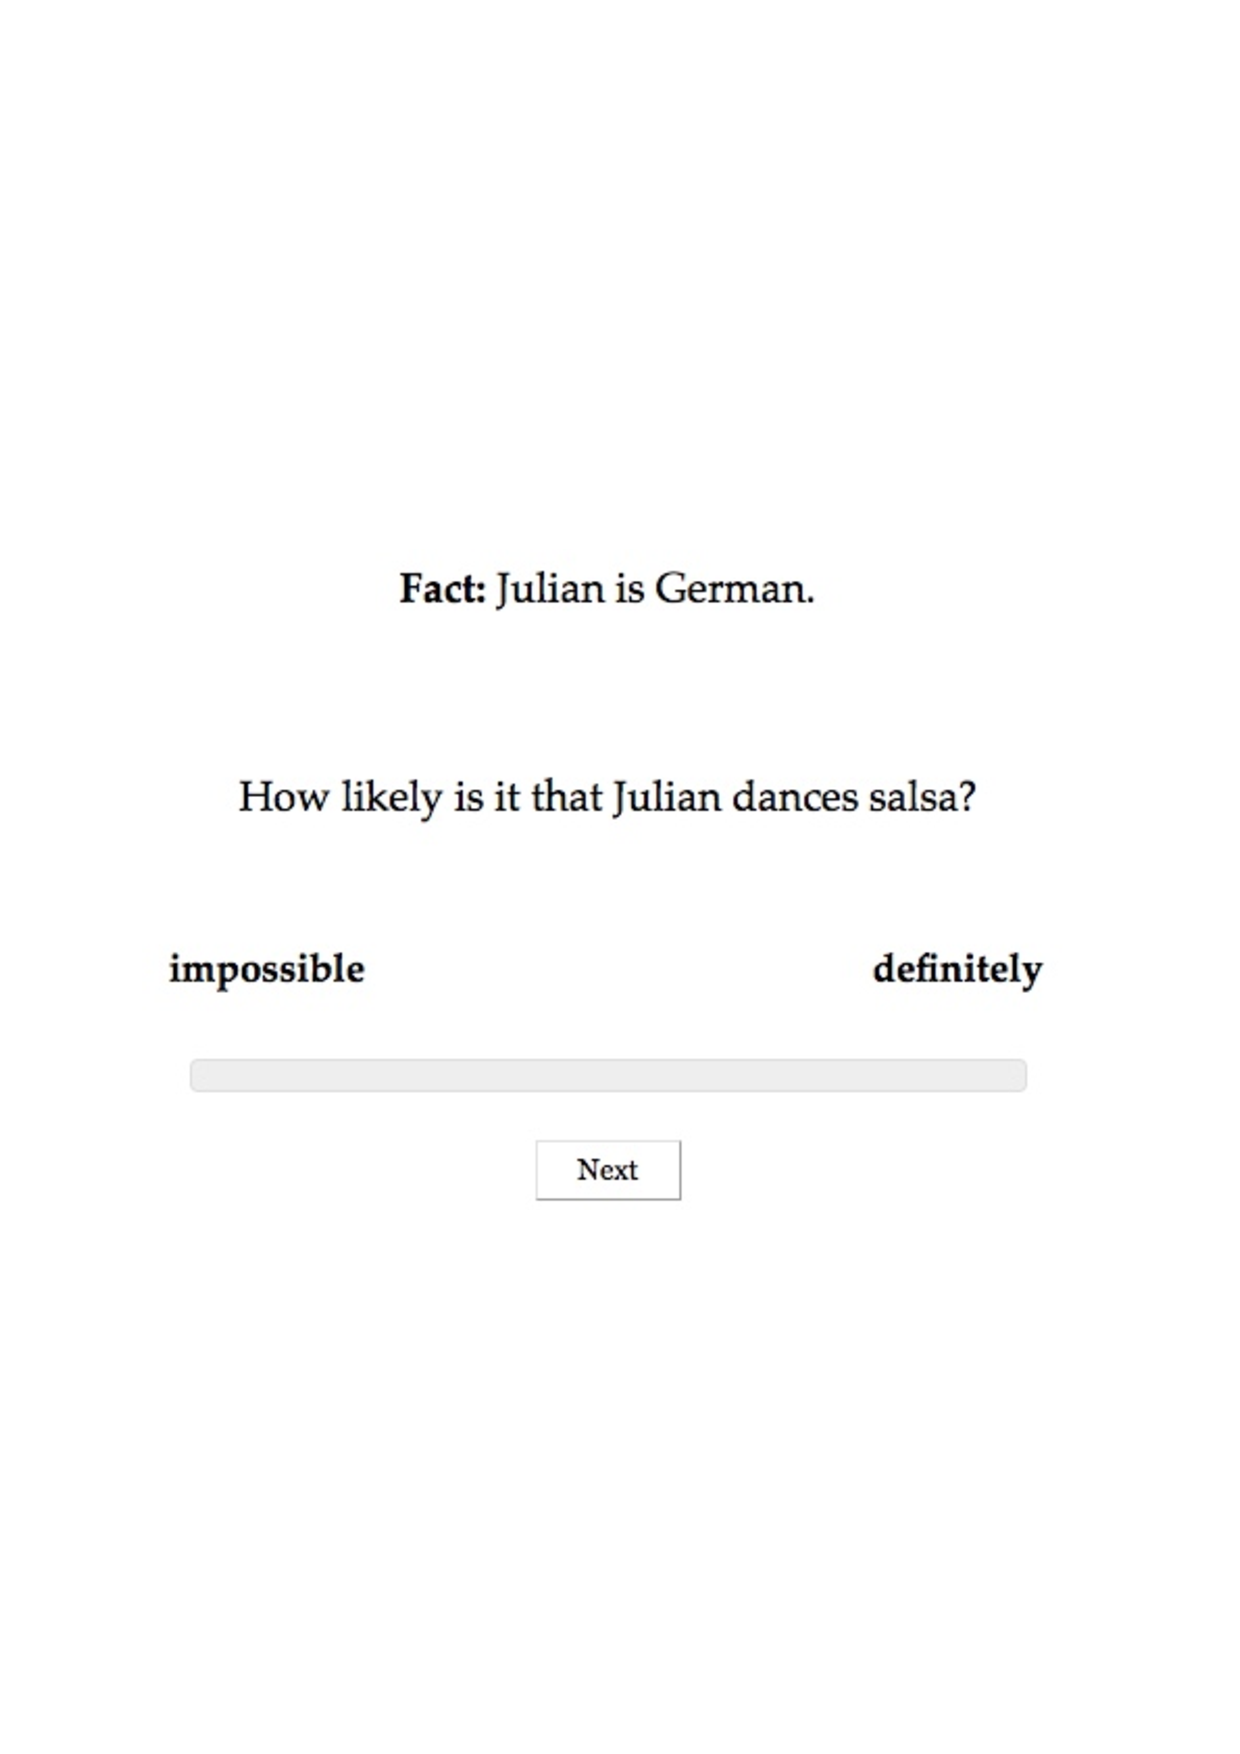
\includegraphics[width=7.6cm]{figures/exp1-prior-trial}}
\caption{Target trial in prior block (`impossible'/low prior coded as 0, `definitely'/high prior coded as 1).}\label{fig-exp1-prior}
\end{subfigure}
 \par\bigskip
\begin{subfigure}[t]{0.8\textwidth}
\par\bigskip
\centering
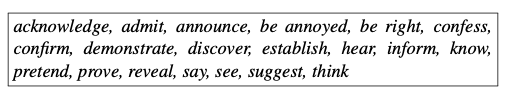
\includegraphics[width=10cm]{figures/predicates}
\caption{20 clause-embedding predicates in the at-issueness and projection blocks.}\label{fig-exp1-predicates}
 \end{subfigure}
 \par\bigskip
\begin{subfigure}[t]{0.5\textwidth}
\par\bigskip
\centering
 \fbox{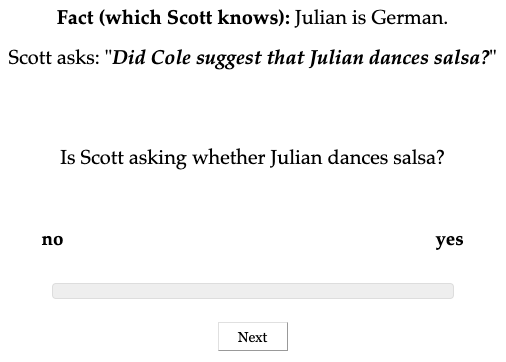
\includegraphics[width=7.6cm]{figures/exp1-nai-trial}} 
\caption{Target trial in at-issueness block (`no'/not-at-issue coded as 1, `yes'/at-issue coded as 0).}\label{fig-exp1-nai}
 \end{subfigure}%
 \hspace*{.3cm} \begin{subfigure}[t]{0.5\textwidth}
\par\bigskip
\centering
 \fbox{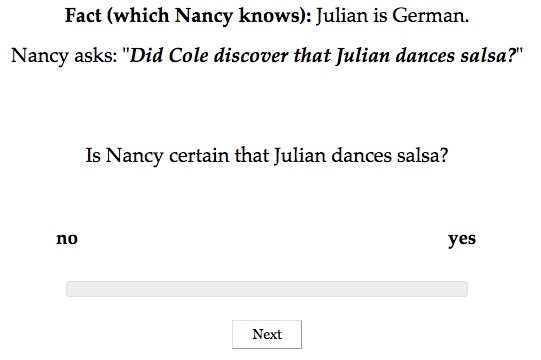
\includegraphics[width=7.6cm]{figures/exp1-projection-trial}} 
\caption{Target trial in projection block (`no'/no projection coded as 0, `yes'/projection coded as 1).}\label{fig-exp1-projection}
 \end{subfigure}

\caption{Sample target trials and clause-embedding predicates in Exp.~1.}
\end{figure}

The at-issueness and projection blocks also included 6 control trials each, which functioned as attention checks: The contents of these items were expected to be at-issue and not to project. The same 6 contents were also used to form 6 filler trials in the prior block. These filler items were not used to assess participants' attention. For the full set of control and filler items see Supplement \ref{a-stim}.

Each participant's set of items was semi-randomly generated: First, the 20 clauses were randomly paired with the 20 predicates. Then, one random half of the items was assigned the respective clause's higher-probability fact, and the other half its lower-probability fact. Participants completed a total of 78 trials: 20 target trials in each block, 6 control trials in the projection and at-issueness blocks each, and 6 filler trials in the prior block. Each participant completed the same filler and control trials.  To measure the prior probability of the contents,  the prior block was presented first to all participants. The projection and at-issueness blocks were then presented in random order. Within blocks, trial order was randomized.

After completing the experiment, participants filled out a short optional demographic survey. To encourage truthful responses, participants were told that they would be paid no matter what answers they gave in the survey.

\paragraph{Data exclusion.} Data was excluded based on self-declared non-native speaker status and other criteria shown in Supplement \ref{a-excl}, leaving 10,100 data points from 505 participants (ages 20-73; mean age: 39.5).

\subsection{Results}\label{s-results-exp1}

We first investigate the relation between prior beliefs, at-issueness, and lexical meaning in modulating projection in section \ref{s:exp1-main-analysis}. To be able to interpret the results, this analysis does not consider interactions between these factors and the order in which the projection and at-issueness blocks were presented to the participants. Instead, we investigate the role of the block order in an auxiliary analysis in section \ref{s:exp1-aux-analysis}.

\subsubsection{Main analysis}\label{s:exp1-main-analysis}

We fit a Bayesian mixed-effects beta regression predicting certainty ratings (measuring projection)\footnote{\label{fn:transform}To model the ratings using a beta regression, the ratings were first transformed from the interval [0,1] to the interval (0,1) using the method proposed in \citealt{smithson-verkuilen2006}.} from a centered fixed effect of asking-whether rating (measuring at-issueness), a centered fixed effect of prior probability rating, a fixed effect of predicate (with treatment coding and {\em prove} as the reference level),\footnote{This reference level was chosen to facilitate the interpretation of the interactions: For {\em prove}, the slope of the fixed effect of asking-whether ratings on certainty ratings was closest to 0.} and the interactions between the fixed effects.\footnote{All analyses were conducted in R (\citealt{R}, version 4.1.2) using the {\tt brms} package (\citealt{buerkner2017}).} The model included random by-content and by-participant intercepts, and random by-content and by-participant slopes for the prior probability and asking-whether fixed effects.\footnote{Models with random by-content and by-participant slopes for predicate and an interaction between the two fixed effect predictors were not run to avoid overfitting the data.} The output of the model included 95\% highest density intervals (HDIs) of means for each fixed effect. We assume that a fixed effect has an effect on certainty ratings (measuring projection) if its HDI does not include 0. Full details of the model outputs are provided in Supplement \ref{a-models-exp1}. 

\begin{figure}[h!]
\centering
\begin{subfigure}[t]{0.49\textwidth}
\centering
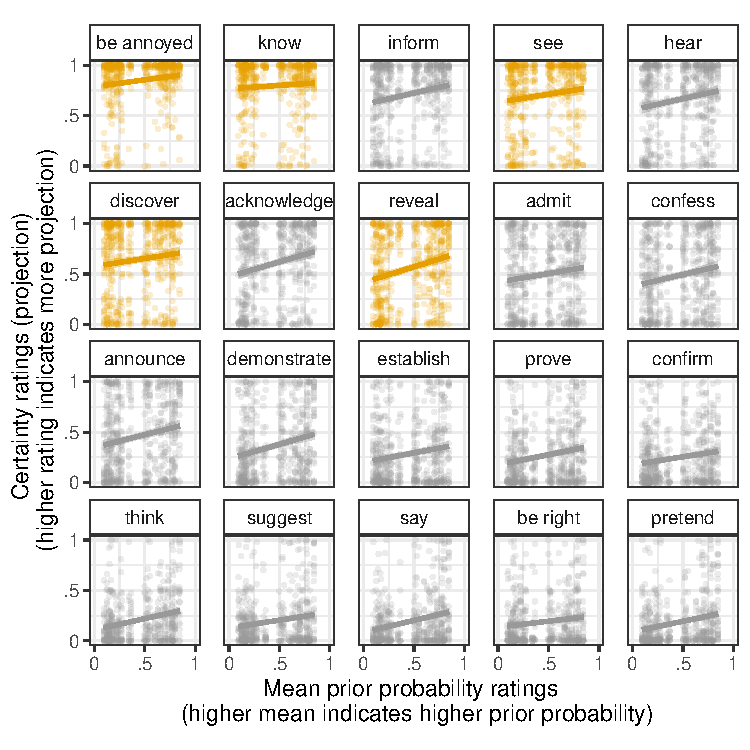
\includegraphics[width=\textwidth]{../../results/main/exp1/graphs/projection-by-prior}
\caption{Certainty against prior probability ratings.}\label{fig:certainty-by-prior}
\end{subfigure} \hfill \begin{subfigure}[t]{0.49\textwidth}
\centering
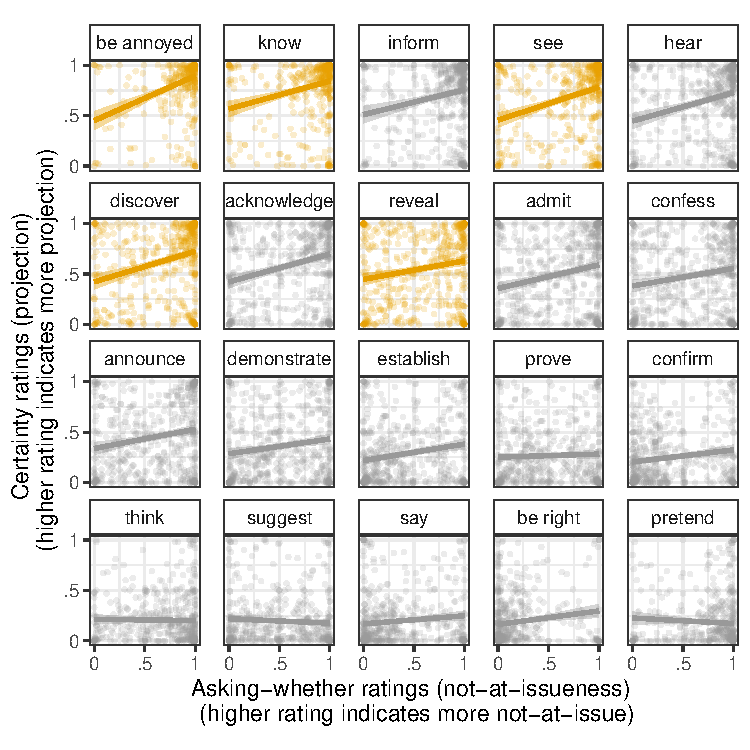
\includegraphics[width=\textwidth]{../../results/main/exp1/graphs/projection-by-ai}
\caption{Certainty against asking-whether ratings.}\label{fig:certainty-by-nai}
 \end{subfigure}
 
\begin{subfigure}[t]{0.49\textwidth}
\centering
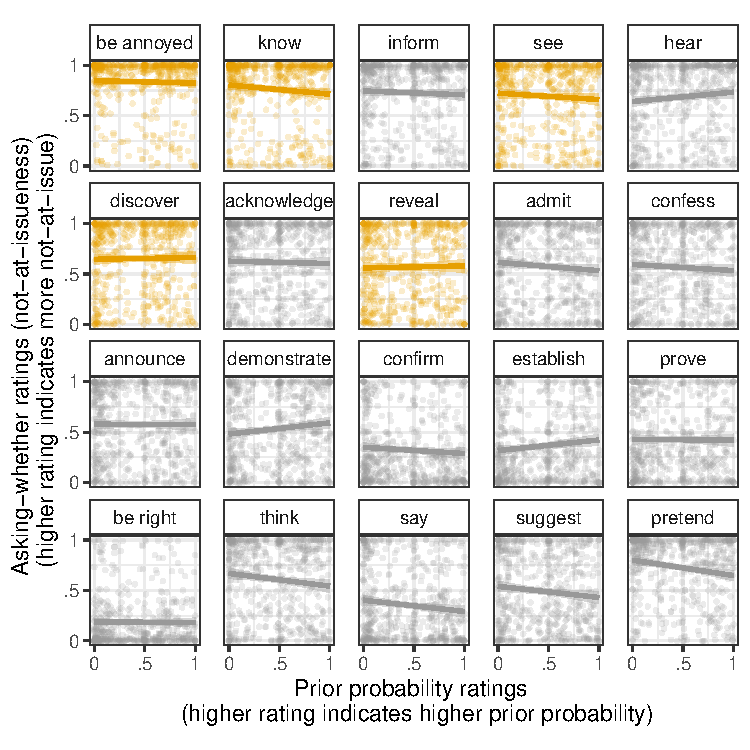
\includegraphics[width=\textwidth]{../../results/main/exp1/graphs/ai-by-prior}
\caption{Asking-whether against prior probability ratings.}\label{fig:ai-by-prior}
\end{subfigure} \hfill 
\begin{subfigure}[t]{0.49\textwidth}
\centering
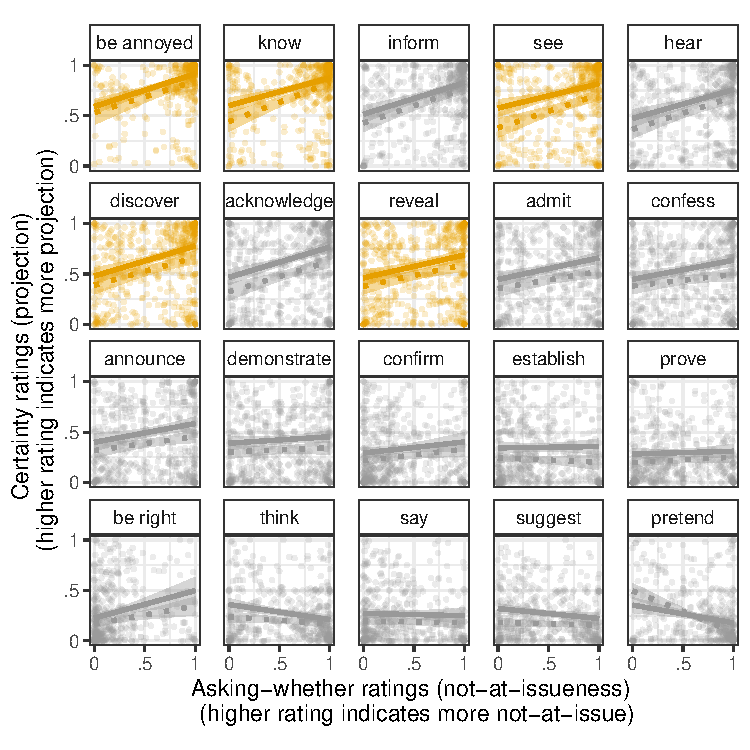
\includegraphics[width=\textwidth]{../../results/main/exp1/graphs/projection-by-ai-and-prior}
\caption{Certainty against asking-whether ratings by high prior probability fact (solid line: ---) and low prior probability fact (dotted line: \raisebox{1mm}{\ldots}).}\label{fig:certainty-by-ai-and-prior}
 \end{subfigure}
  
\caption{Participants' ratings in Exp.~1 (full dataset) by predicate: (a) certainty ratings (measuring projection) against prior probability ratings, (b) certainty ratings (measuring projection) against asking-whether ratings (measuring projection), (c) certainty ratings (measuring projection) against asking-whether ratings (measuring at-issueness) by high and low prior probability fact. Linear smoothers with 95\% confidence intervals overlaid. Predicates are ordered by projection mean, with purportedly factive predicates in orange.}\label{fig:results1}
\end{figure}

\paragraph{(I) The relation between prior beliefs and lexical meaning in modulating projection.} Recall that \citealt{degen-tonhauser-openmind} observed a positive effect of prior probability on projection: The higher an interpreter's prior belief in a content, the more the interpreter takes the speaker to believe in the content. This result is replicated in the current experiment: As shown in Fig.~\ref{fig:certainty-by-prior}, which shows participants' prior probability ratings against their certainty ratings (measuring projection) by clause-embedding predicate,\footnote{The predicates are ordered in Figs.~\ref{fig:results1} and \ref{fig:results2} by the strength of the projection of the CC in the respective experiment.} there is a positive effect for each predicate, suggesting that the higher an interpreter's prior belief about content, the more the content projects.

These observations were supported by the model: The HDI for the main effect of the prior at the reference level {\em establish} did not contain 0 ($\beta$ = 1, [.65-1.34]), which suggests that, for the CC of {\em establish}, the higher the prior probability rating, the higher the certainty rating is. The HDI for the interactions between the other predicates and the prior contained 0, which suggests that the effect of the prior for the CC of these predicates does not differ from that of {\em establish}. In other words, for these predicates, too, the higher an interpreter's prior belief in a content, the more the interpreter takes the speaker to believe in the content.\footnote{Exp.~1 also replicates a result from \citepos{degen-tonhauser-language} Exp.~1a and \citepos{degen-tonhauser-openmind} Exp.~1, namely the effect of the meanings of the 20 predicates on the projection of the CC; for Spearman rank correlations and visualizations see Supplement \ref{a-replication}).} 
                          
\paragraph{(II) The relation between at-issueness and lexical meaning in modulating projection.} Recall that \citepos{tbd-variability} Gradient Projection Principle leads us to expect a positive effect of not-at-issueness on projection for all predicates. \citepos{djaerv-bacovcin2020} analysis, on the other hand, predicts a positive effect only for factive predicates and no effect for non-factive ones. Fig.~\ref{fig:certainty-by-nai} shows participants' certainty ratings (measuring projection) against asking-whether ratings (measuring not-at-issueness) by clause-embedding predicate: There is a positive effect for most predicates (e.g., {\em know, inform, announce, acknowledge}), no effect for some predicates (e.g., {\em prove, confirm}), and a negative one for others (e.g., {\em pretend, think}). 

The observations were supported by the model: The HDI for the main effect of at-issueness at the reference level {\em prove} contained 0 ($\beta$ = .06, [0,.13]), which suggests that, for the CC of {\em prove}, there is no effect of at-issueness on projection. For 12 of the other predicates (namely {\em acknowledge, admit, announce, be annoyed, be right, confess, discover, hear, inform, know, reveal, see}), the coefficient was positive and the HDIs for the interactions between the predicates and at-issueness did not contain 0. This suggests that, for these predicates, there was an effect of at-issueness on projection, such that the more not-at-issue the CC was, the more it projected. For three predicates (namely {\em pretend, suggest, think}), the coefficient was negative and the HDIs for the interactions between the predicates and at-issueness did not contain 0. This suggests that, for these predicates, there was an effect of at-issueness on projection such that the more at-issue the CC was, the more it projected. Finally, there were four predicates besides {\em prove} (namely {\em confirm, demonstrate, establish, say}) for which the HDIs for the interactions between the other predicates and at-issueness contained 0. This suggests that, for these predicates, as for \emph{prove}, there was no effect of at-issueness on projection. 

These observations are neither completely predicted by the Gradient Projection Principle (which does not lead us to expect predicates with a non-positive effects, like {\em prove} or {\em think}) nor by \citepos{djaerv-bacovcin2020} analysis (which does not lead us to expect non-factive predicates with positive effects, like {\em admit} or {\em acknowledge}).


\paragraph{(III) The relation between prior beliefs and at-issueness in modulating projection.} Recall that \citepos{tonhauser-etal-eval} Non-redundancy Principle for At-issue Content predicts a positive effect of prior beliefs on not-at-issueness, whereas extant RSA models of projection inferences assume no relation between the two factors. Fig.~\ref{fig:ai-by-prior} shows participants asking-whether ratings (measuring at-issueness) by prior probability rating. 


Fig.~\ref{fig:certainty-by-ai-and-prior} shows participants' certainty ratings (measuring projection) against asking-whether ratings (measuring at-issueness) by prior probability and by predicate. There is no relation for most predicates, but some predicates seem to exhibit a negative relation (e.g., {\em pretend, suggest, say, think}) and others a positive one (e.g., {\em establish, demonstrate, hear}). The model, however, does not confirm any of these interactions: The HDI for the interaction between prior probability and at-issueness at the reference level {\em prove} contains 0 ($\beta$ = .05, [-.14,.24]), which suggests that, for the CC of {\em prove}, there is no interaction between prior beliefs and at-issueness in modulating projection. The HDIs for the interactions between the other predicates, prior probability and at-issueness also contained 0, which suggests that there was no effect of the prior on at-issueness for any of these predicates in modulating projection either.  These results provide support for the assumption made in extant RSA models that there is no relation between prior beliefs and at-issueness in modulating projection (\citealt{qing-etal2016,stevens-etal2017,warstadt2022,pan-degen2023}) and contrary to \citepos{tonhauser-etal-eval} Non-redundancy Principle for At-issue Content.

\subsubsection{Auxiliary block order analysis}\label{s:exp1-aux-analysis}

In order to assess the role that block order may have played in the results reported above, we conducted a block order analysis. To this end, we fit the model reported above to two separate subsets of the data depending on whether the  projection block preceded or followed the at-issueness block. Supplement \ref{a-models-exp1} contains the full details of these models' outputs. The results of the analysis fit to the entire dataset and of the analyses fit to the two subsets are summarized in the first three columns of Table \ref{t:results}.

\newpage

\setlength{\fboxrule}{0pt}
\setlength{\tabcolsep}{4.5pt}
%\begin{landscape}
\begin{table}[h!]
\centering
\input{../../results/main/exp1/models/latex-tables/t1}

\input{../../results/main/exp1/models/latex-tables/t1AIPRIOR}
\caption{Summary of the results of Exps.~1-4: the `Factor' column identifies the factor and the `Experiment' column the experiment and whether the model was fit to the entire dataset (`full data'), the subset in which the projection block came first (`proj/ai'), or the subset in which the at-issueness block came first (`ai/proj'). Predicates ordered by mean projection in Exp.~1 with factive predicates in \color{orange}orange\color{black}. Color coding indicates whether the effect was positive (red) or negative (blue), and the Bayes factor of the effect:
\\ \hspace*{1cm} \colorbox{red1}{\makebox[1em][c]{\framebox[1em]{\rule{0pt}{3pt}}}},\colorbox{blue1}{\makebox[1em][c]{\framebox[1em]{\rule{0pt}{3pt}}}}: 21+ (``very strong to extreme evidence'')
\\ \hspace*{1cm} \colorbox{red2}{\makebox[1em][c]{\framebox[1em]{\rule{0pt}{3pt}}}},\colorbox{blue2}{\makebox[1em][c]{\framebox[1em]{\rule{0pt}{3pt}}}}: 11-20 (``strong evidence'')
%\\ \hspace*{1cm} \colorbox{red3}{\makebox[1em][c]{\framebox[1em]{\rule{0pt}{3pt}}}},\colorbox{blue3}{\makebox[1em][c]{\framebox[1em]{\rule{0pt}{3pt}}}}: 11-20 (``strong evidence'')
\\ \hspace*{1cm} \colorbox{red4}{\makebox[1em][c]{\framebox[1em]{\rule{0pt}{3pt}}}},\colorbox{blue4}{\makebox[1em][c]{\framebox[1em]{\rule{0pt}{3pt}}}}: 2-10 (``weak to moderate evidence'')
%\\ \hspace*{1cm} \colorbox{red5}{\makebox[1em][c]{\framebox[1em]{\rule{0pt}{3pt}}}},\colorbox{blue5}{\makebox[1em][c]{\framebox[1em]{\rule{0pt}{3pt}}}}: 2-5 (``weak evidence'')
\\ A white box means that there was no evidence for an effect.
}

\label{t:results}
\end{table}
%\end{landscape}

\newpage

%\begin{table}[H]
%\begin{subtable}[t]{\textwidth}
%\centering
%\input{../../results/main/exp1/models/latex-tables/priorTable}
%\caption{Effect of prior probability ratings on certainty ratings, by predicate}
%\end{subtable}
%
%\begin{subtable}[t]{\textwidth}
%\centering
%\input{../../results/main/exp1/models/latex-tables/aiTable}
%\caption{Effect of asking whether ratings on certainty ratings, by predicate}
%\end{subtable}

%\begin{subtable}[t]{\textwidth}
%\centering
%\input{../../results/main/exp1/models/latex-tables/pAITable}
%\caption{Effect of asking whether ratings and prior ratings on certainty ratings, by predicate}
%\end{subtable}
%
%\caption{Summary of the results of Exps.~1 and 2, by predicate: (a) effect of prior probability on certainty ratings, (b) effect of at-issueness on certainty ratings, (c) effect of the interaction between prior probability and at-issueness on certainty ratings. The columns distinguish between whether the model was fit to the entire dataset (`full data'), the subset in which the at-issueness block came first (`ai/proj'), or the subset in which the projection block came first (`proj/ai'). Predicates ordered by mean projection in Exp.~1 with factive predicates in \color{orange}orange\color{black}. 
%\newline
%Positive coefficients: \colorbox{green1}{\makebox[4em][c]{$>=.95$}}, \colorbox{green2}{\makebox[4em][c]{[$.85,.95)$}}, 
%\colorbox{green3}{\makebox[4em][c]{[$.75,.85)$}}, 
%\colorbox{green4}{\makebox[4em][c]{$<.75$}}; \newline negative coefficients: \colorbox{yellow1}{\makebox[4em][c]{$>=.95$}}, \colorbox{yellow2}{\makebox[4em][c]{[$.85,.95)$}}, 
%\colorbox{yellow3}{\makebox[4em][c]{[$.75,.85)$}}, 
%\colorbox{yellow4}{\makebox[4em][c]{$<.75$}}}
%\label{t:results}
%\end{table}

\newpage

%\begin{table}[h!]
%\centering
%\begin{tabular}{l | ccc | ccc | c | c}
%& \multicolumn{8}{c}{\bf Experiment/Dataset} \\ 
%
% & \multicolumn{3}{c|}{\bf Exp.~1} & \multicolumn{3}{c|}{\bf Exp.~2} &  {\bf Exp.} &  {\bf Exp.} \\ 
%
%  & full & ai/ & proj/ & full & ai/ & proj/ & {\bf DT1} & {\bf DT2} \\ 
%{\bf Factors modulating projection} & data & proj & ai & data & proj & ai & & \\ 
%
%
%\midrule
%
%(indiv./mean) prior beliefs *  & \multirow{2}{*}{$\checkmark$} &  \multirow{2}{*}{$\bullet$} & \multirow{2}{*}{$\checkmark$} & \multirow{2}{*}{$\checkmark$}  &  \multirow{2}{*}{$\bullet$} & \multirow{2}{*}{$\checkmark$} & \multirow{2}{*}{$\checkmark$} & \multirow{2}{*}{$\checkmark$} \\ 
%\hspace*{2.3cm} each of the 20 predicates  & & & & & & & \\ 
%
%\hline
%
%(indiv./mean) at-issueness * \emph{acknowledge} & $\checkmark^+$  & $\checkmark^+$ & $\checkmark^+$  & $\checkmark^+$ & $\checkmark^+$ & $\checkmark^+$ & $\bullet$ &  $\bullet$\\ 
%
%\hspace*{4.3cm}\emph{admit} & $\checkmark^+$ & $\checkmark^+$& $\checkmark^+$  & $\checkmark^+$  &$\checkmark^+$ & $\checkmark^+$ & $\bullet$ & $\bullet$\\ 
%
%\hspace*{4.3cm}\emph{announce} & $\checkmark^+$ & $\checkmark^+$& $\checkmark^+$  & $\checkmark^+$ & $\checkmark^+$& $\bullet$ & $\bullet$& $\checkmark^+$\\ 
%
%\hspace*{4.3cm}\emph{be annoyed} & $\checkmark^+$ & $\checkmark^+$& $\checkmark^+$  & $\checkmark^+$ & $\checkmark^+$& $\checkmark^+$ & $\bullet$& $\bullet$\\ 
%
%\hspace*{4.3cm}\emph{be right} & $\checkmark^+$ & $\checkmark^+$& $\checkmark^+$  & $\checkmark^+$ & $\checkmark^+$& $\bullet$ & $\bullet$& $\bullet$\\ 
%
%\hspace*{4.3cm}\emph{confess} & $\checkmark^+$ & $\checkmark^+$& $\checkmark^+$  & $\checkmark^+$ & $\checkmark^+$& $\bullet$ & $\bullet$&$\bullet$ \\ 
%
%\hspace*{4.3cm}\emph{confirm} & $\bullet$ & $\bullet$ & $\checkmark^+$  & $\bullet$ & $\bullet$& $\bullet$ & $\bullet$& $\bullet$\\ 
%
%\hspace*{4.3cm}\emph{demonstrate} & $\bullet$ & $\bullet$ & $\checkmark^+$  & $\bullet$ & $\bullet$ & $\bullet$ & $\bullet$& $\bullet$\\ 
%
%\hspace*{4.3cm}\emph{discover} & $\checkmark^+$ & $\checkmark^+$& $\checkmark^+$ & $\checkmark^+$ & $\checkmark^+$ & $\checkmark^+$ & $\bullet$&$\checkmark^+$ \\ 
%
%\hspace*{4.3cm}\emph{establish} & $\bullet$& $\bullet$ & $\checkmark^+$  & $\checkmark^+$ & $\checkmark^+$ & $\bullet$ & $\bullet$&$\bullet$ \\ 
%
%\hspace*{4.3cm}\emph{hear} & $\checkmark^+$ & $\checkmark^+$& $\checkmark^+$  & $\checkmark^+$ & $\checkmark^+$& $\checkmark^+$ & $\bullet$& $\bullet$\\ 
%
%\hspace*{4.3cm}\emph{inform} & $\checkmark^+$ & $\checkmark^+$& $\checkmark^+$  & $\checkmark^+$ & $\checkmark^+$& $\checkmark^+$ & $\bullet$&$\bullet$ \\ 
%
%\hspace*{4.3cm}\emph{know} & $\checkmark^+$ & $\checkmark^+$& $\checkmark^+$  & $\checkmark^+$ & $\checkmark^+$& $\checkmark^+$ & $\bullet$& $\bullet$\\ 
%
%\hspace*{4.3cm}\emph{pretend} & $\checkmark^{-}$ & $\checkmark^-$& $\checkmark^-$  & $\bullet$  & $\bullet$ & $\bullet$ & $\bullet$& $\bullet$\\ 
%
%\hspace*{4.3cm}\emph{prove} & $\bullet$ & $\bullet$ & $\checkmark^+$  & $\bullet$  & $\bullet$& $\bullet$ & $\bullet$& $\bullet$\\ 
%
%\hspace*{4.3cm}\emph{suggest} & $\checkmark^{-}$ & $\bullet$ & $\checkmark^{-}$ & $\bullet$& $\bullet$ & $\bullet$ & $\bullet$&$\bullet$ \\ 
%
%\hspace*{4.3cm}\emph{reveal} & $\checkmark^+$ & $\checkmark^+$ & $\checkmark^+$  & $\checkmark^+$  & $\bullet$ & $\checkmark^+$ & $\bullet$& $\bullet$\\ 
%
%\hspace*{4.3cm}\emph{say} &$\bullet$ & $\bullet$ & $\checkmark^+$  & $\bullet$ & $\bullet$ & $\bullet$ & $\bullet$& $\bullet$\\ 
%
%\hspace*{4.3cm}\emph{see} & $\checkmark^+$ & $\checkmark^+$& $\checkmark^+$  & $\checkmark^+$ & $\checkmark^+$ & $\checkmark^+$ & $\bullet$& $\checkmark^+$\\ 
%
%\hspace*{4.3cm}\emph{think} & $\checkmark^{-}$ & $\bullet$ & $\checkmark^{-}$  & $\bullet$ & $\bullet$ & $\bullet$ & $\bullet$ & $\checkmark^+$ \\ 
%
%\hline
%
%(indiv./mean) prior beliefs * & \multirow{2}{*}{$\bullet$} & \multirow{2}{*}{$\bullet$} & \multirow{2}{*}{$\bullet$} & \multirow{2}{*}{$\bullet$} & \multirow{2}{*}{$\bullet$}& \multirow{2}{*}{$\bullet$} & \multirow{2}{*}{$\bullet$}  & \multirow{2}{*}{$\bullet$} \\ 
%\hspace*{2cm} (indiv./mean) at-issueness & & & & & & & &  \\ 
%
%\bottomrule
%\end{tabular}
%\caption{Summary of the results of Exp.~1 and the three partial replications. For Exps.~1 and 2, the three columns distinguish between whether the model was fit to the entire dataset (`full data'), the subset in which the at-issueness block came first (`ai/proj'), or the subset in which the projection block came first (`proj/ai'). A checkmark ($\checkmark$) means that the factor significantly modulated projection, a bullet ($\bullet$) means that it did not. In the 20 rows for the effect of at-issueness and the predicates, the superscripts on the checkmarks ($\checkmark\textsuperscript{--}, \checkmark\textsuperscript{+}$) identify whether the coefficient was negative or positive.}\label{t:results}
%\end{table}


\paragraph{(I) The relation between prior beliefs and lexical meaning in modulating projection.} The order of the blocks mattered for the relation between prior beliefs and lexical meaning in modulating projection. The model fit to the subset of the data where the projection block immediately followed the prior block (`proj/ai' in Table \ref{t:results}) suggests that there is an effect of prior beliefs on projection for every predicate, just like the model fit to the entire dataset.  However, the model fit to the subset of the data where the at-issueness block intervened between the prior and projection blocks (`ai/proj' in Table \ref{t:results}) did not support an effect of prior beliefs on projection for any predicate, though the coefficient was positive for every predicate except {\em be right, inform}, and {\em pretend}. 

\paragraph{(II) The relation between at-issueness and lexical meaning in modulating projection.} The order of the blocks mattered for the relation between at-issueness and lexical meaning in modulating projection. As summarized in Table \ref{t:results}, the model fit to the subset of the data where the at-issueness block preceded the projection block does not support a negative effect of not-at-issueness and projection for {\em suggest} and {\em think}. And the model fit to the subset of the data where the projection block preceded the at-issueness block supports a positive effect between not-at-issueness and projection for a larger set of predicates than the model fit to the full dataset (namely also for {\em confirm, demonstrate, establish, prove} and {\em say}). 

\paragraph{(III) The relation between prior beliefs and at-issueness in modulating projection.} The order in which the blocks were presented to the participants did not have an effect on the relation between prior beliefs and at-issueness in modulating projection. As shown in Table \ref{t:results}, the models fit to the two subsets do not support such a relation for any predicate, just like the model fit to the entire dataset.

\subsection{Discussion}\label{s:discussion-exp1}

The results of Exp.~1 replicate the results of prior research --- that prior beliefs, at-issueness, and lexical meaning modulate projection --- and provide insight into the relations between these factors. Regarding (I) the relation between prior beliefs and lexical meaning in modulating projection, the model fit to the full dataset suggests that there is an effect of prior beliefs on projection that persists across the lexical meanings of the 20 clause-embedding predicates. While this effect came out in the subset of the data in which the projection block immediately followed the prior block, it did not in the subset of the data in which the at-issueness block intervened between the prior block and the projection block. One possible explanation is that the effect of prior beliefs on projection is an artifact of the design of Exp.~1, such that participants' certainty ratings on the projection block are artificially influenced by their prior belief ratings, but only when the prior blick immediately precedes the projection block. Another possible explanation is that the effect of prior beliefs on projection is real, but when the at-issueness block directly precedes the projection block, participants' attention is drawn to the question of what the speaker is asking about, thereby drawing resources away from integrating information from the prior. One way of distinguishing these explanations is to collect certainty ratings from a set of participants who did not also provide prior belief ratings and using a separate group's prior belief ratings as a predictor of these certainty ratings. This is what we will do in Exp.~2, which is reported on in the next section. Preliminary support for the latter explanation comes from \citepos{degen-tonhauser-openmind} Exp.~2, which suggested that there is an effect of prior beliefs on projection even when the prior belief ratings were collected from a different set of participants than the projection ratings (but the contribution of lexical meaning was not considered in that work).

Regarding (II) the relation between at-issueness and lexical meaning in modulating projection, the models fit to the full dataset and the two subsets suggest that there is a systematic effect of at-issueness on projection for some predicates. Specifically, for {\em acknowledge, admit, announce,  be annoyed, be right, confess, discover, hear, establish, inform, know, reveal} and {\em see}, Exp.~1 suggests that the more not-at-issue the CC of these predicates is, the more it projects. This result is not in line with \citepos{djaerv-bacovcin2020} analysis, as it leads us to expect this relation only for factive predicates, not for nonfactive ones. While the results for these predicates are in line with \citepos{tbd-variability} Gradient Projection Principle, there are also predicates whose lexical meaning does not appear to interact with at-issueness in the way that is expected from the Gradient Projection Principle. The lexical meaning of {\em pretend}, for instance, appears to interact with at-issueness in the opposite way, such that the more not-at-issue the CC is, the less it projects; this is also suggested for {\em think} and {\em suggest}, at least by the model fit to the full dataset and the subset in which the at-issueness block follows the projection block. And the lexical meaning of predicates like {\em confirm, demonstrate, establish, prove}, and {\em say} appears to only show the effect expected by the Gradient Projection Principle when the at-issueness block follows the projection block. To understand whether these interactions between lexical meaning and at-issueness replicate, we ran Exp.~2. A discussion of the theoretical implications of the results is postponed to section \ref{s4}.

Finally, regarding (III) the relation between prior beliefs and at-issueness, the analyses of the entire dataset of Exp.~1 and of the two subsets suggests that these two factors do not interact in modulating projection. This result is in line with what is assumed in extant RSA models of projection inferences (\citealt{qing-etal2016,stevens-etal2017,warstadt2022,pan-degen2023}) and contrary to \citepos{tonhauser-etal-eval} Non-redundancy Principle for At-issue Content, which assumed that the higher the a priori belief in a content is, the less at-issue it is. 

\section{Partial replications of Exp.~1}\label{s3}

This section reports on the results of Exp.~2, which had the same design as Exp.~1 except that there was no prior block, as shown in Table \ref{t:overview}. We added to Exp.~2 the mean prior probability ratings of the 40 content/fact combinations pooled from Exp.~1, the prior block of Exp.~DT1, and Exp.~DT2a. By adding mean prior probability ratings from a separate set of participants, Exp.~2 allows us to investigate an open question from Exp.~1, namely whether the effect of prior beliefs on projection is real or an artifact of the design of Exp.~1. By collecting certainty and asking-whether ratings in a within-participant design, Exp.~2 allows us to further investigate another open question from Exp.~1, namely whether the interactions between lexical meaning and at-issueness replicate. 



the results of three analyses of experiments that each partially replicates Exp.~1. The ways in which each of the three experiments partially replicates Exp.~1 are shown in Table \ref{t:overview}. Exp.~2 had the same design as Exp.~1 except that prior probability ratings were not collected (i.e., there was no prior block). Exp.~1 from \citealt{degen-tonhauser-openmind} (henceforth `Exp.~DT1') had the same design as Exp.~1 except that asking-whether ratings were not collected (i.e., there was no at-issueness block). Finally, Exp.~2 from \citealt{degen-tonhauser-openmind} (henceforth `Exp.~DT2') had the same design as Exp.~1 except that there was no at-issueness block, and the prior and projection blocks of Exp.~1 were run as separate experiments.

\begin{table}[h]
\centering
\begin{tabular}{l || c | c | c | c}
& \multicolumn{4}{c}{\bf Experiment} \\ 
{\bf Ratings collected} & Exp.~1 & Exp.~2 & Exp.~DT1 & Exp.~DT2 \\ \hline\hline

Certainty & $\Smiley$ & $\Smiley$ & $\Smiley$ & $\Smiley$ (Exp.~DT2a) \\

Asking whether & $\Smiley$ & $\Smiley$ & -- & -- \\

Prior probability & $\Smiley$ & -- & $\Smiley$ & $\Smiley$ (Exp.~DT2b) \\

\end{tabular}
\caption{Ratings collected in Exp.~1, Exp.~2, and Exps.~DT1 and DT2 (Exps.~1 and 2 from \citealt{degen-tonhauser-openmind}). A smiley ($\Smiley$) means that a rating was collected; a minus (--) means that it was not.}\label{t:overview}
\end{table}

Each of the replications differed from Exp.~1 in that some rating was not collected. To investigate the relation between prior beliefs, at-issueness, and lexical meaning in modulating projection inferences, we added the missing ratings to the datasets of the replications. Specifically, we added to Exp.~2 the mean prior probability ratings of the 40 content/fact combinations pooled from Exp.~1, the prior block of Exp.~DT1, and Exp.~DT2a, and we added to Exps.~DT1 and DT2 the mean asking-whether ratings of the 800 content/fact/predicate combinations pooled from Exps.~1 and 2.\footnote{Supplement \ref{a-beliefs-corr-prior} compares the mean prior probabilities of the 40 content/fact combinations in the three experiments. Supplement \ref{a-beliefs-corr-ai} compares the mean asking-whether ratings of the 800 content/fact/predicate combinations in Exps.~1 and 2. We return to these in the general discussion in section \ref{s4}.}


\subsection{Experiment 2}\label{s:exp2}

Exp.~2 was identical to Exp.~1 except that the prior block was omitted.

\subsubsection{Methods}

\paragraph{Participants.} 600 participants with U.S.\ IP addresses and at least 99\% of previous HITs approved were recruited on Amazon's Mechanical Turk platform (ages: 19-73, median: 37.5). They were paid \$2.20.\footnote{92 individuals participated in both experiments. Since the experiments were run four months apart (Exp.~1: December 16, 2019; Exp.~2: August 21, 2019), it is unlikely that these participants' responses were primed by their prior participation.}

\paragraph{Materials and procedure.}  Exp.~2 differed from Exp.~1 only in that there was no prior block. As in Exp.~1, each participant's set of items was semi-randomly generated: First, the 20 clauses were randomly paired with the 20 predicates. Then, one random half of the items was assigned the respective clause's higher-probability fact, and the other half its lower-probability fact. Participants completed a total of 52 trials: 20 target trials in each block, and 6 control trials in the projection and at-issueness blocks each. Each participant completed the same control trials. The projection and at-issueness blocks were presented in random order. 

\paragraph{Data exclusion.} Data was excluded based on self-declared non-native speaker status and other criteria shown in Supplement \ref{a-excl}, leaving 10,160 data points from 508 participants (ages 19-73; mean age: 38.3).

\subsubsection{Results}

We fit a Bayesian mixed-effects linear regression predicting participants' certainty ratings (measuring projection) from a centered fixed effect of participants' asking-whether rating (measuring at-issueness), a centered fixed effect of by-content/fact mean prior probability rating, a fixed effect of predicate (with treatment coding and {\em prove} as the reference level), and the interactions between the fixed effects. The model included random by-content and by-participant intercepts, and random by-content and by-participant slopes for the prior probability and asking-whether fixed effects. As with Exp.~1, we did not include a fixed effect for block to be able to interpret the critical interactions between at-issueness, prior beliefs, and lexical meaning. Instead, the data were split up by whether the projection block preceded or followed the at-issueness block, and the same model that was fit to the full dataset was fit to these two sub-datasets. Full details of the outputs of the three models are provided in Supplement \ref{a-models-exp2}. 

%\begin{exe}
%\ex Exp (ai/proj)
%\begin{xlist}
%\ex prior: no effect of prior on projection for {\em prove} (positive coefficient), ns interaction with other predicates (all positive coefficients, except for {\em discover, hear, inform, know, see, suggest, think})
%\ex ai: as with data pooled, except that $\bullet$ for {\em reveal} instead of $\checkmark^{+}$
%\item prior*ai: as with data pooled, except for {\em reveal, be annoyed}, both negative coefficient
%\end{xlist}
%\ex Exp (proj/ai)
%\begin{xlist}
%\ex prior: as with data pooled
%\ex ai: as with data pooled, except that {\em announce, be right, confess, establish} are not  $\checkmark^{+}$ but $\bullet$
%\item prior*ai: as with data pooled, except for {\em announce} (positive coefficient)
%\end{xlist}
%\end{exe}

\paragraph{The relation between prior beliefs and lexical meaning in modulating projection.} In contrast to Exp.~1, where prior belief ratings were collected in a within-participant design, the prior belief ratings in Exp.~2 were by-content/fact mean ratings pooled from Exp.~1, DT1, and DT2a. As shown in Fig.~\ref{fig:certainty-by-prior2}, which shows by-content/fact  prior probability means against by-content/fact certainty means (measuring projection) by clause-embedding predicate, there is a positive correlation for each predicate. This observation was supported by the model that was fit to the full dataset: The HDI for the main effect of the prior at the reference level {\em prove} did not contain 0 ($\beta$ = .18, [.08,.28]), which suggests that, for the CC of {\em prove}, the higher the by-content/fact mean prior probability rating, the higher the participants' certainty rating is. The HDIs for the interactions between the other predicates and the prior contained 0, which suggests that the effect of the prior for the CC of these predicates does not differ from that of {\em prove}. In other words, we observe for all 20 predicates that the higher the by-content/fact mean prior probability is, the more the interpreter takes the speaker to believe in the content.

We observe the same effect of block order in Exp.~2 as in Exp.~1: As summarized in Table \ref{t:results}, the model fit to the subset of the data in which the at-issueness block precedes the projection block does not support an effect of prior beliefs on projection (though the coefficient is again positive for most predicates). However, the model fit to the subset of the data in which the projection block precedes the at-issueness block does support the effect of prior beliefs on projection that is also supported by the model fit to the full dataset. We take this to provide support for the second explanation for the block effect proposed in section \ref{s:discussion-exp1}: There is an effect of prior beliefs on projection, but this effect is masked when the at-issueness block immediately precedes the projection block.

\begin{figure}[h!]
\centering
\begin{subfigure}[t]{0.49\textwidth}
\centering
\includegraphics[width=\textwidth]{../../results/main/exp2/graphs/means-projection-by-prior}
\caption{Certainty ratings against prior probability ratings.}\label{fig:certainty-by-prior2}
\end{subfigure} \hfill \begin{subfigure}[t]{0.49\textwidth}
\centering
\includegraphics[width=\textwidth]{../../results/main/exp2/graphs/d-projection-by-ai}
\caption{Certainty ratings against asking-whether ratings.}\label{fig:certainty-by-nai2}
 \end{subfigure}
 
\begin{subfigure}[t]{0.49\textwidth}
\centering
\includegraphics[width=\textwidth]{../../results/main/exp2/graphs/means-ai-by-prior}
\caption{At-issueness ratings against prior probability ratings.}\label{fig:ai-by-prior2}
 \end{subfigure}
 
\caption{Ratings in Exp.~2, by predicate: (a) by-content/fact mean certainty ratings against mean prior probability ratings, (b) participants' certainty ratings against asking-whether ratings, (c) by-content/fact mean asking-whether ratings against prior probability ratings. Predicates ordered by projection mean in Exp.~2. Linear smoothers with 95\% confidence intervals overlaid.}\label{fig:results2}
\end{figure}

\paragraph{The relation between at-issueness and lexical meaning in modulating projection.} At-issueness and projection ratings were collected in a within-participant design in Exp.~2, just like in Exp.~1. The by-predicate variation in the effect of at-issueness on projection observed in Exp.~1 is also observed in Exp.~2, as shown in Fig.~\ref{fig:certainty-by-nai2}, which shows participants' certainty ratings (measuring projection) against asking-whether ratings (measuring not-at-issueness) by clause-embedding predicate: There is a positive correlation for some predicates (e.g., {\em be annoyed, announce}) and no correlation for others (e.g., {\em think}). These observations were supported by the model fit to the full dataset: The HDI for the main effect of at-issueness at the reference level {\em prove} contained 0 ($\beta$ = .04, [-.03,.11]), which suggests that, for the CC of {\em prove}, there is no effect of at-issueness on projection. For 13 of the other predicates (namely {\em acknowledge, admit, announce, be annoyed, be right, confess, discover, establish, hear, inform, know, reveal, see}), the coefficient was positive and the HDIs for the interactions between the other predicates and at-issueness did not contain 0. This suggests that, for these predicates, there was an effect of at-issueness on projection, such that the more not-at-issue the CC was, the more it projected. For the remaining six predicates (namely {\em confirm, demonstrate, pretend, say, suggest, think}), the HDIs for the interactions between the other predicates and at-issueness contained 0. This suggests that, for these predicates, as for \emph{prove}, there was no effect of at-issueness on projection. 

As in Exp.~1, there was an effect of block order on the relation between at-issueness and lexical meaning in modulating projection: As summarized in Table \ref{t:results}, the model fit to the subset of the data in which the at-issueness block preceded the projection block did not support a positive correlation between not-at-issueness and projection for {\em reveal}, and the model fit to the subset of the data in which the projection block preceded the at-issueness block did not support a positive correlation for {\em announce, be right, confess}, and {\em establish}. Thus, the model fit to the full dataset of Exp.~2 supported a positive correlation between not-at-issueness and projection for a larger set of predicates than each of the subsets. There are also differences between Exps.~1 and 2: First, the set of predicates for which there was a positive correlation between not-at-issueness and projection (in line with the Gradient Projection Principle) was slightly larger in Exp.~2 than in Exp.~1. Second,  there is no predicate for which the models fit to the Exp.~2 data support a negative correlation between not-at-issueness and projection. For the predicates for which such a negative correlation was supported in Exp.~1, the Exp.~2 data suggest that there is no correlation.

\paragraph{The relation between prior beliefs and at-issueness in modulating projection.} Recall that Exp.~1 found no relation between individual participants' prior probability ratings and their asking-whether ratings (measuring at-issueness) in modulating their certainty ratings (measuring projection), in line with extant RSA models of projection. Exp.~2 suggests that this result also holds at the group level, that is, that by-content/fact prior probability means do not interact with participants' asking-whether ratings in modulating their certainty ratings. As shown in Fig.~\ref{fig:ai-by-prior2}, which shows by-content/fact asking-whether means (measuring at-issueness) against by-content/fact prior probability means by clause-embedding predicate, there is no relation for any predicate. This observation is confirmed by the model: The HDI for the interaction between prior probability and at-issueness at the reference level {\em prove} contains 0 ($\beta$ = .01, [-.15,.34]), which suggests that, for the CC of {\em prove}, there is no interaction between group-level prior beliefs and at-issueness. Furthermore, the HDIs for the interactions between the other predicates, prior probability and at-issueness also contained 0, which suggests that there was no effect of the prior on at-issueness for any of these predicates either. 

There was an effect of block order: The model fit to the subset of the data in which the at-issueness block preceded the projection block supports a negative relation between prior beliefs and not-at-issueness for {\em reveal} and {\em be annoyed}, and the model fit to the other subset supports a positive relation for {\em announce}. We ignore these interactions as neither is supported by the model fit to the full dataset. In sum, while the results of Exp.~1 provide support for the assumption made in extant RSA models of projection that there is no relation between interpreters' prior beliefs and at-issueness in modulating projection, the results of Exp.~2 strengthen the support for this assumption by showing that there is no relation between group-level prior beliefs and at-issueness either.

\subsection{Experiments DT1 and DT2 (Experiments 1 and 2 from \citealt{degen-tonhauser-openmind})}\label{s:OMExps}

The next two partial replications are based on Exps.~DT1 and DT2: As noted above, these experiments followed the design of Exp.~1 except that there was no at-issueness block and, in Exp.~DT2, separate sets of participants provided the prior probability and certainty ratings.

We fit a Bayesian mixed-effects linear regression predicting participants' certainty ratings to both of  datasets. For Exp.~DT1, the fixed effects included a centered fixed effect of mean asking-whether ratings, a centered fixed effect of participants' prior probability rating, a fixed effect of predicate (with treatment coding and {\em acknowledge} as the reference level),\footnote{As with Exps.~1 and 2 above, this reference level was chosen to facilitate the interpretation of the interactions.} and the three way-interaction between fixed effects. The model included random by-content and by-participant intercepts, and random by-content and by-participant slopes for the prior probability and asking-whether fixed effects. For Exp.~DT2, the fixed effects were the same as for Exp.~DT1 except that the prior predictor was based on mean rather than individual prior probability ratings. Full details of the model output are provided in Supplement \ref{a-models-OM}.

\paragraph{The relation between prior beliefs and lexical meaning in modulating projection.} For Exp.~DT1, the HDI for the main effect of the prior at the reference level {\em acknowledge} did not contain 0 ($\beta$ = .26, [.13,.39]), which suggests that, for the CC of {\em acknowledge}, the higher the by-content/fact mean prior probability rating, the higher the participants' certainty rating is. The HDIs for the interactions between the other predicates and the prior contained 0, suggesting that there is a positive relation between prior beliefs and projection for these predicates, too. The only exception was {\em think} ($\beta$ = .24, [.05,.43]), where the positive coefficient suggests that the positive relation between prior beliefs and projection was stronger than for the other predicates. This result replicates that of Exp.~1, where prior and projection ratings were also collected in a within-participant design.

For Exp.~DT2, the HDI for the main effect of the prior mean at the reference level {\em acknowledge} did not contain 0 ($\beta$ = .37, [.2,.54]), which suggests that, for the CC of {\em acknowledge}, the higher the by-content/fact mean prior probability rating, the higher the participants' certainty rating is. The HDIs for the interactions between the other predicates and the prior contained 0, suggesting that for these predicates, too, the higher the group-level belief in the content, the more the content projects. This result replicates that of Exp.~2, where prior and projection ratings were also collected in a between-participant design.

\paragraph{The relation between at-issueness and lexical meaning in modulating projection.} For Exp.~DT1, the HDI for the main effect of mean at-issueness at the reference level {\em acknowledge} contained 0 ($\beta$ = .12, [-.39,.63]), which suggests that, for the CC of {\em acknowledge}, there is no effect of at-issueness on projection. For the other 19 predicates, too, the HDIs for the interactions between the other predicates and at-issueness contained 0. This suggests that there is no effect of mean at-issueness on projection for any of the 20 predicates. 

For Exp.~DT2, the HDI for the main effect of mean at-issueness at the reference level {\em acknowledge} also contained 0 ($\beta$ = -.41, [-.96,.15]), suggesting, again, that, for the CC of {\em acknowledge}, there is no effect of at-issueness on projection (though note that the coefficient here is negative, whereas it was positive for Exp.~DT1). For four predicates (namely {\em announce, discover, see, think}), the coefficient was positive and the HDI did not contain 0. This suggests that, for these four predicates, the higher the mean not-at-issueness is, the more the CC projects. For the remaining 15 predicates, the HDIs for the interactions between the other predicates and at-issueness contained 0, suggesting again that there is no effect of at-issueness on projection for these predicates.

\paragraph{The relation between prior beliefs and at-issueness in modulating projection.} For Exp.~DT1, the HDI for the interaction between participants' prior probability ratings and mean at-issueness ratings at the reference level {\em acknowledge} contains 0 ($\beta$ = -.54, [-2.24,1.07]), which suggests that, for the CC of {\em acknowledge}, there is no interaction between individual prior beliefs and group-level at-issueness. Furthermore, the HDIs for the interactions between the other predicates, participants' prior probability ratings and mean at-issueness ratings also contained 0, except for {\em hear}, which suggests that there is no support for an effect of prior beliefs on at-issueness. 

For Exp.~DT2, the HDI for the interaction between mean prior probability ratings and mean at-issueness ratings at the reference level {\em acknowledge} contains 0 ($\beta$ = -.44, [-2.38,1.41]), which suggests that, for the CC of {\em acknowledge}, there is no interaction between individual prior beliefs and group-level at-issueness. Furthermore, the HDIs for the interactions between the other predicates, mean prior probability ratings and mean at-issueness ratings also contained 0, which suggests that there is no support for an effect of prior beliefs on at-issueness.

\subsubsection{Summary}

The results of Exp.~1 suggested that (I) the effect of prior beliefs on projection persists across predicates, (II) there is by-predicate variation in the effect of at-issueness on projection, and (III) prior beliefs and at-issueness do not interact in modulating projection. Whereas (III) was supported regardless of the order in which the at-issueness and projection blocks were presented to the participants, an effect of block order was observed for (I) and (II). The three partial replications of Exp.~1 were able to provide insight into how reliable these results are.



As shown in Table \ref{t:results}, there was no support for a relation between prior beliefs and at-issueness in modulating projection regardless of whether certainty ratings were predicted from individual-level prior belief and at-issueness ratings (Exp.~1), group-level prior belief and individual-level at-issueness ratings (Exp.~2), individual-level prior belief and group-level at-issueness ratings (Exp.~DT1), or group-level prior belief and at-issueness ratings (Exp.~DT2). These results provide strong support for the assumption, made in extant RSA models of projection inferences, that there is no relation between prior beliefs and at-issueness in modulating projection (\citealt{qing-etal2016,stevens-etal2017,warstadt2022,pan-degen2023}), contrary to \citepos{tonhauser-etal-eval} Non-redundancy Principle for At-issue Content.

For the relation between prior beliefs and lexical meaning in modulating projection, there was support for the assumption that certainty ratings are predicted from individual-level prior belief ratings (Exps.~1 and DT1) and from group-level prior belief ratings  (Exps.~2 and DT2) and that both of these results hold across the 20 predicates. This was not true only for those subsets of the data in which the at-issueness block immediately preceded the projection block, regardless of whether the prior belief ratings were obtained from the same individuals (Exp.~1) or from a separate set of individuals (Exp.~2). We take this to mean that prior beliefs modulate projection across clause-embedding predicates, but that the effect can be masked by other factors. 

Finally, the summary in Table \ref{t:results} suggests that the relation between at-issueness and lexical meaning in modulating projection depends on whether projection is predicted from individual-level at-issueness ratings (Exps.~1 and 2) or from group-level at-issueness ratings (Exps.~DT1 and DT2). In the former case, there is support for a positive correlation between not-at-issueness and projection for many predicates and no correlation (or a negative one) for some. In the latter case, however, there is no support for a consistent effect of at-issueness on projection regardless of the predicate. To understand why the results differ depending on whether we consider individual-level or group-level at-issueness ratings, it is instructive to compare the asking-whether ratings obtained in Exps.~1 and 2. As shown in Fig.~\ref{fig:ai-comparisons}, the asking whether ratings for the 800 combinations of a predicate, a content, and a fact obtained in Exp.~2 are not positively correlated with those obtained in Exp.~1.

This lack of a positive correlation may be due to there being noise in the data, though note that the design and analyses of Exps.~1 and 2 mitigated against such noise, by presenting the same 20 predicates in the same sentence structures and combining them with the same complement clauses across participants, by presenting all utterances in the same context, and by obtaining ratings from a large number of participants, whose response variability was taken into consideration in the statistical analyses. We therefore consider it unlikely that the variation is due to noise. Rather, we hypothesize that the variation is due to the information that was available to the participants (see Fig.~\ref{fig-exp1-nai}) being insufficient to render a stable asking-whether rating. Specifically, we hypothesize that more stable asking-whether ratings could be obtained by presenting spoken utterances rather than written ones. This hypothesis is motivated by the assumption that the prosodic realization of an utterance provides a cue to the Question Under Discussion addressed by the utterance, which in turn identifies which content is at-issue.

The 800 group-level at-issueness means that were added to the datasets of Exps.~DT1 and DT2 were obtained by aggregating the asking-whether ratings for the 800 combinations of a predicate, a content, and a fact of Exps.~1 and 2. This means that the group-level at-issueness ratings added to the datasets of Exps.~DT1 and DT2 reflected neither the group-level means of Exp.~1 nor of Exp.~2. So, within-participant ratings work (presumably same implicit prosody) but group-level ratings don't work unless prosody is controlled, or at-issueness is measured better.

What about the difference between Exp.1 and 2? We can take away that (a) there is by-predicate variation, and (b) there are predicates with positive correlation and predicates with no correlation. Whether there are predicates with negative correlation...

\section{General discussion}\label{s4}

\begin{itemize}

\item (I) prior beliefs

\item(II) \citealt{stevens-etal2017,tonhauser-etal-sub23}

Finally, our experiment revealed that a content's at-issueness does not invariably modulate projection of the content.  This result is consistent with the results of \citealt{cummins-rohde2015}, which point to variability among 19 presupposition triggers, including 6 factive predicates, and the results of \citealt{djaerv-bacovcin-salt27, djaerv-bacovcin2020} and \citealt{mahler-etal2020}, which identify differences between factive predicates (where the results were consistent with the Gradient Projection Principle) and non-factive predicates (where they were not). The variation observed in our experiment does not confirm this distinction between factive and non-factive predicates: For instance, the positive correlation between not-at-issueness and projection was observed not just for factive {\em know} but also for non-factive {\em announce} and {\em be right}; furthermore, there was no correlation for some non-factive predicates (e.g., {\em say}) and a negative one for others (e.g., {\em think}). As the formal model proposed in \citealt{djaerv-bacovcin2020} assumes that the  variation is between factive and non-factive predicates, this model cannot capture the variation observed in our experiment (see also the challenges to the assumption that there is a class of factive predicates raised in \citealt{degen-tonhauser-language}).

A predictive model of projection inferences must include a systematic account of this interaction. We hypothesize that (yet to be identified) components of lexical meaning constrain whether the projection of the content of the clausal complement is modulated by the question under discussion. For instance, an analysis according to which the lexical meaning of {\em pretend} entails that the speaker is committed to the falsity of the content of the complement predicts that this content does not project even when it is not at-issue. Which components of lexical meaning play a role in modulating projection inferences is an important question for future research.

\item (III) The main result of the experiment reported on in this paper suggests that these two factors independently modulate projection inferences, rather than at-issueness being constrained by, or even reducible to, interpreters' prior beliefs about the content (cf.\ \citealt{tonhauser-etal-eval}). 

This result provides empirical support for formal models of projection inferences that acknowledge the independent contribution of these two factors, such as the RSA models of \citealt{qing-etal2016} and \citealt{stevens-etal2017}. Neither of these models straightforwardly extend to the projection inferences investigated in our experiment: They are designed for projection inferences triggered by change-of-state verbs like \emph{stop} (\citealt{qing-etal2016}) or by utterances' prosody (\citealt{stevens-etal2017}) and therefore do not capture the variable contributions of the lexical meanings of the clause-embedding predicates to projection inferences. Developing such an RSA analysis is a pressing task for future research.

\end{itemize}

\section{Conclusions}\label{s5}

\section*{Data accessibility statement}

The experiments, data, and R code for generating the figures and analyses reported on in this paper are available at [link redacted for review]
%\href{https://github.com/judith-tonhauser/attitude\_preds\_projection}{https://github.com/judith-tonhauser/attitude\_preds\_projection}
.  Exps.~1 and 2 were preregistered at [link redacted for review].
%\href{https://osf.io/tg2bn}{https://osf.io/tg2bn}.

\section*{Ethics and consent}

The experiment was declared exempt from review by the IRB of [university redacted for review]. Informed consent was obtained from the participants.

% uncomment for word count
%\end{document}

%\section*{Acknowledgments}
%(removed for review)

\bibliographystyle{cslipubs-natbib}
%\bibliographystyle{apacite}
\bibliography{bibliography}

% uncomment for word count
%\end{document}

\newpage

\appendix

\setcounter{table}{0}
\renewcommand{\thetable}{A\arabic{table}}

\setcounter{figure}{0}
\renewcommand{\thefigure}{A\arabic{figure}}

\section*{Supplements}

\section{Target and control items}\label{a-stim}

\paragraph{Target items} This list shows the 20 clauses of the target items with their lower and higher probability facts, respectively:

\begin{enumerate}[leftmargin=4ex,itemsep=-2pt]
\item Mary is pregnant. Facts: Mary is a middle school student / Mary is taking a prenatal yoga class
\item Josie went on vacation to France. Facts:  Josie doesn't have a passport / Josie loves France 
\item Emma studied on Saturday morning. Facts: Emma is in first grade / Emma is in law school 
\item Olivia sleeps until noon. Facts: Olivia has two small children / Olivia works the third shift
\item Sophia got a tattoo. Facts: Sophia is a high end fashion model / Sophia is a hipster
\item Mia drank 2 cocktails last night. Facts: Mia is a nun / Mia is a college student
\item Isabella ate a steak on Sunday. Facts: Isabella is a vegetarian / Isabella is from Argentina
\item Emily bought a car yesterday. Facts: Emily never has any money / Emily has been saving for a year
\item Grace visited her sister. Facts: Grace hates her sister / Grace loves her sister
\item Zoe calculated the tip. Facts: Zoe is 5 years old / Zoe is a math major
\item Danny ate the last cupcake. Facts: Danny is a diabetic / Danny loves cake
\item Frank got a cat. Facts: Frank is allergic to cats / Frank has always wanted a pet
\item Jackson ran 10 miles. Facts: Jackson is obese / Jackson is training for a marathon
\item Jayden rented a car. Facts: Jayden doesn't have a driver's license / Jayden's car is in the shop
\item Tony had a drink last night. Facts: Tony has been sober for 20 years / Tony really likes to party with his friends
\item Josh learned to ride a bike yesterday. Facts: Josh is a 75-year old man / Josh is a 5-year old boy
\item Owen shoveled snow last winter. Facts: Owen lives in New Orleans / Owen lives in Chicago
\item Julian dances salsa. Facts: Julian is German / Julian is Cuban
\item Jon walks to work. Facts: Jon lives 10 miles away from work / Jon lives 2 blocks away from work
\item Charley speaks Spanish. Facts: Charley lives in Korea / Charley lives in Mexico
\end{enumerate}

In the target items of the projection and at-issueness blocks, eventive predicates, like {\em discover} and {\em hear}, were realized in the past tense and stative predicates, like {\em know} and {\em be annoyed}, were realized in the present tense. The direct object of {\em inform} was realized by the proper name {\em Sam}. Each clause-embedding predicate was paired with a unique subject proper name. The speaker of the target items was realized by a randomly sampled unique proper name. 

\paragraph{Control and filler items} The not-at-issueness and projection blocks included 6 control trials each. The full set of control items is given in (\ref{control-items}). The content of these items was expected to be at-issue and not to project: For example, (\ref{control-items}f) the speaker is asking about the main clause content, that is, whether Samantha has a new hat, and the speaker is not committed to the main clause content, that Samantha has a new hat. The same 6 main clauses were also used to form 6 filler trials in the prior block. These filler items were not used to assess participants' attention. 

\begin{exe}
\ex\label{control-items}
\begin{xlist}
\ex Do these muffins have blueberries in them? Fact: Muffins are sold at the bakery. 
\ex Does this pizza have mushrooms on it? Fact: Pizza is sold at the pizzeria.
\ex Was Jack playing outside with the kids? Fact: Many children like ice cream.
\ex Does Ann dance ballet? Fact: Ballet is a type of dance.
\ex Were Carl's kids in the garage? Fact: Garages are used to store cars and other things.
\ex Does Samantha have a new hat? Fact: Hats are worn on the head.
\end{xlist}
\end{exe}

\section{Data exclusion}\label{a-excl}

\paragraph{Exp.~1.} We excluded the data from 16 participants who did not self-identify as native speakers of American English. We also excluded the data from one participant who always clicked on the same point of the scale across the target trials, as well as the data from 78 participants whose response means on the 6 not-at-issueness and projection control items were was more than 2 sd above the group means. 

\paragraph{Exp.~2.} We excluded the data from 27 participants who did not self-identify as native speakers of American English. We also excluded the data from 5 participants who always clicked on the same point of the scale across the target trials, as well as the data from 60 participants whose response means on the 6 not-at-issueness and projection control items were was more than 2 sd above the group means. 


\section{Manipulation of prior beliefs in Exp.~1}\label{a-beliefs-exp1}

\figref{f-prior} shows the mean prior probability ratings of the 20 contents by fact from Exp.~1. As shown, contents presented with the higher probability fact received higher prior probability ratings than contents presented with the lower probability fact. This result is confirmed by a mixed-effects linear regression model that predicts prior probability slider ratings from dummy-coded fact type (reference level: `lower probability') and random by-content and by-participant intercepts and slopes for fact type.  The content's mean prior probability was rated as higher when it was presented with its higher probability fact than when it was presented with its lower probability fact ($\beta$ = 0.51, $SE$ = 0.03, $t$ = 17.41, $p$ $<$ .0001). This result suggests that the manipulation of the prior probability of the 20 contents was successful.

\begin{figure}[h!]
\centering
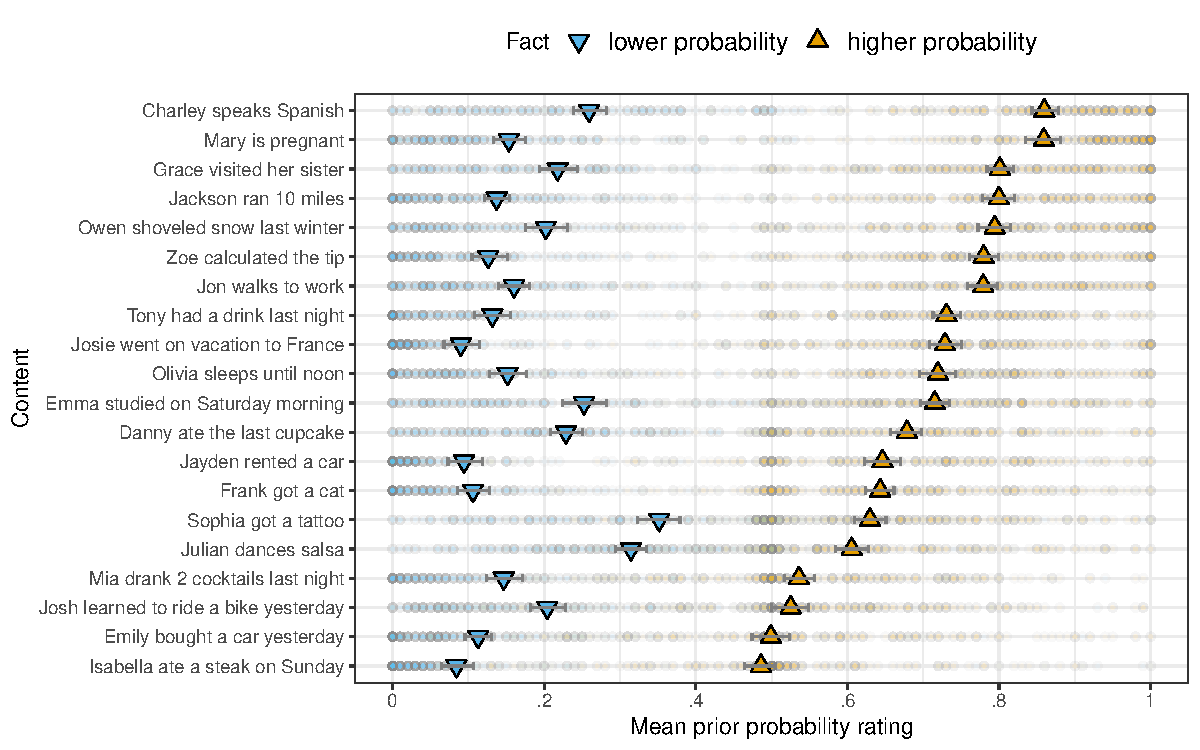
\includegraphics[width=.7\paperwidth]{../../results/main/exp1/graphs/prior-ratings}

\caption{Mean prior probability rating by content and fact in Exp.~1. Error bars indicate 95\% bootstrapped confidence intervals. Transparent dots indicate individual participant ratings.} 
\label{f-prior}
\end{figure}

\newpage

\section{Exp.~1: Results by block order}

The figures in this section present the results by block order, with the results for the two blocks side-by-side.

\subsection{Certainty against prior probability ratings}

\begin{figure}[h!]
\centering
\begin{subfigure}[t]{0.49\textwidth}
\centering
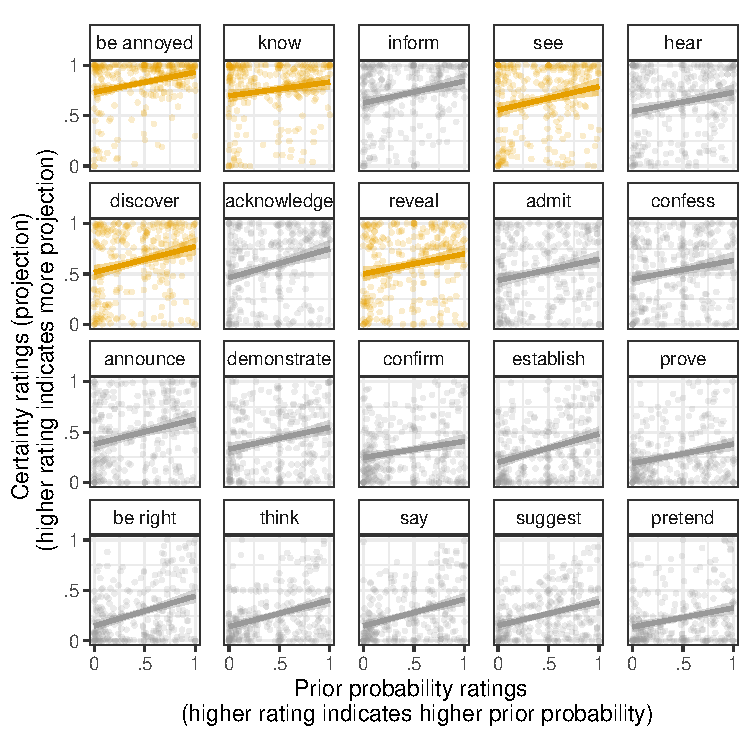
\includegraphics[width=.9\textwidth]{../../results/main/exp1/graphs/SUP-projai-projection-by-prior}
\caption{Proj/ai dataset.}
\end{subfigure} \hfill \begin{subfigure}[t]{0.49\textwidth}
\centering
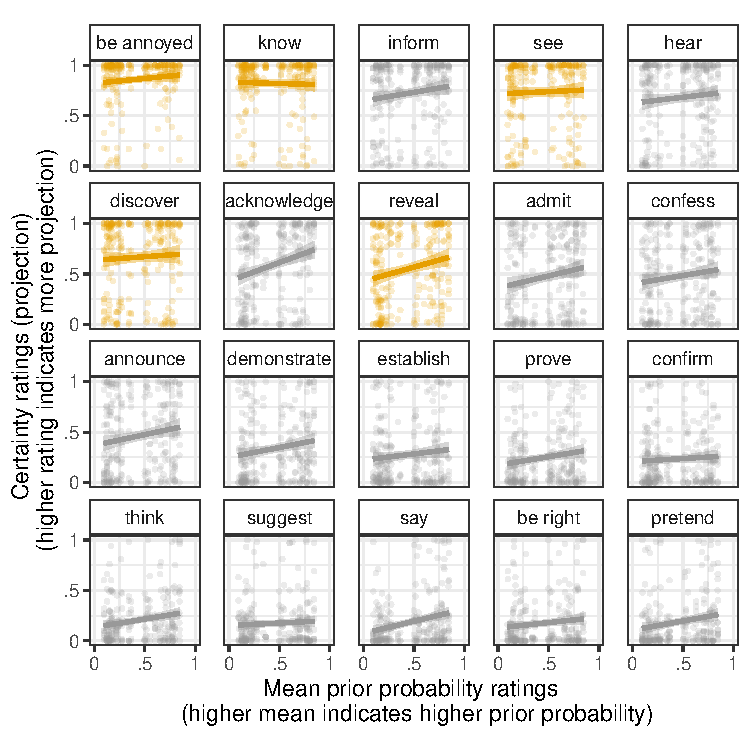
\includegraphics[width=.9\textwidth]{../../results/main/exp1/graphs/SUP-aiproj-projection-by-prior}
\caption{Ai/proj dataset.}
 \end{subfigure}
 
  
\caption{Participants' certainty ratings (measuring projection) against prior probability ratings in Exp.~1: (a) Proj/ai dataset, (b) Ai/proj dataset. Linear smoothers with 95\% confidence intervals overlaid. Predicates are ordered by projection mean, with purportedly factive predicates in orange.}
\end{figure}

\newpage

\subsection{Certainty against asking-whether ratings}

\begin{figure}[h!]
\centering
\begin{subfigure}[t]{0.49\textwidth}
\centering
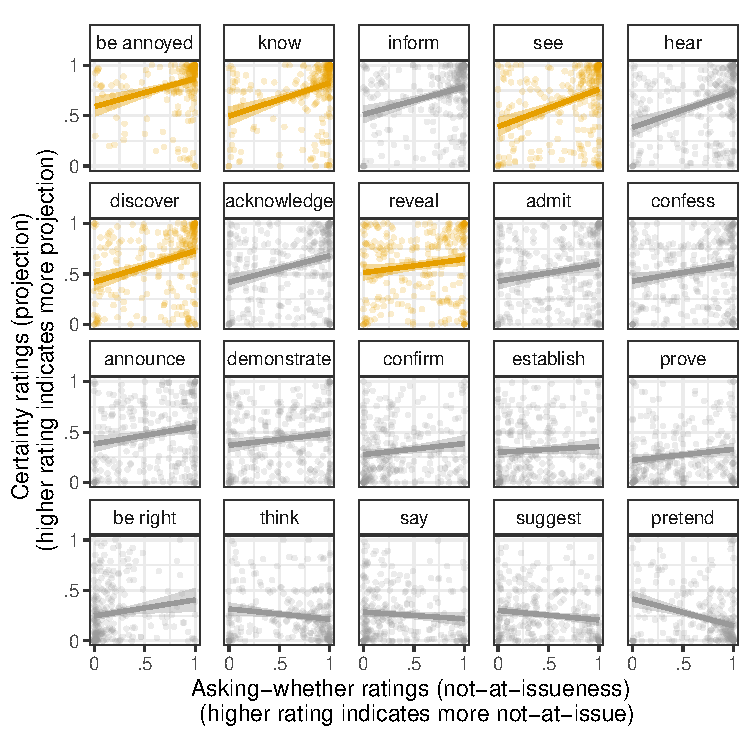
\includegraphics[width=.9\textwidth]{../../results/main/exp1/graphs/SUP-projai-projection-by-ai}
\caption{Proj/ai dataset.}
\end{subfigure} \hfill \begin{subfigure}[t]{0.49\textwidth}
\centering
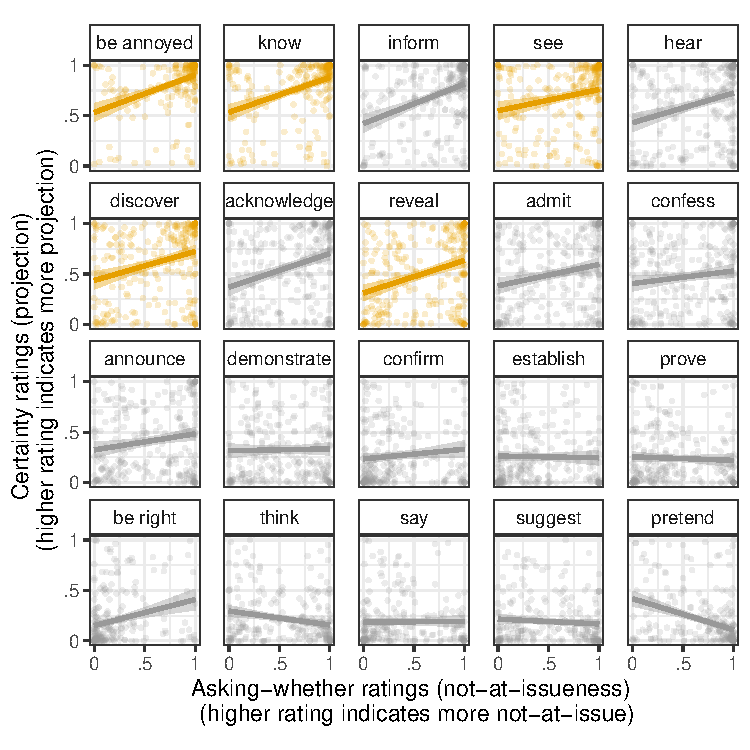
\includegraphics[width=.9\textwidth]{../../results/main/exp1/graphs/SUP-aiproj-projection-by-ai}
\caption{Ai/proj dataset.}
 \end{subfigure}
 
  
\caption{Participants' certainty ratings (measuring projection) against asking-whether ratings (measuring projection) in Exp.~1: (a) Proj/ai dataset, (b) Ai/proj dataset. Linear smoothers with 95\% confidence intervals overlaid. Predicates are ordered by projection mean, with purportedly factive predicates in orange.}
\end{figure}

\subsection{Asking-whether against prior probability ratings}

\begin{figure}[h!]
\centering
\begin{subfigure}[t]{0.49\textwidth}
\centering
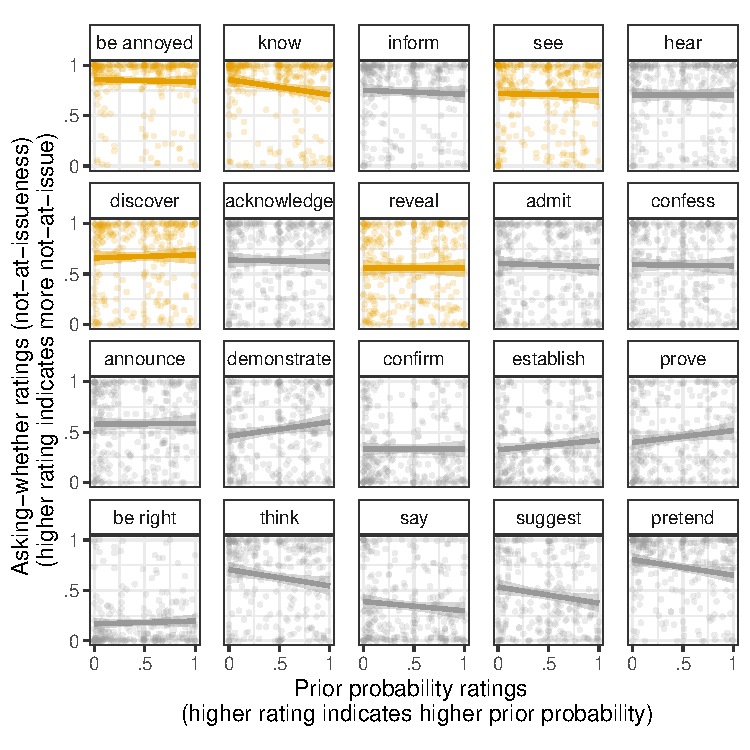
\includegraphics[width=.9\textwidth]{../../results/main/exp1/graphs/SUP-projai-ai-by-prior}
\caption{Proj/ai dataset.}
\end{subfigure} \hfill \begin{subfigure}[t]{0.49\textwidth}
\centering
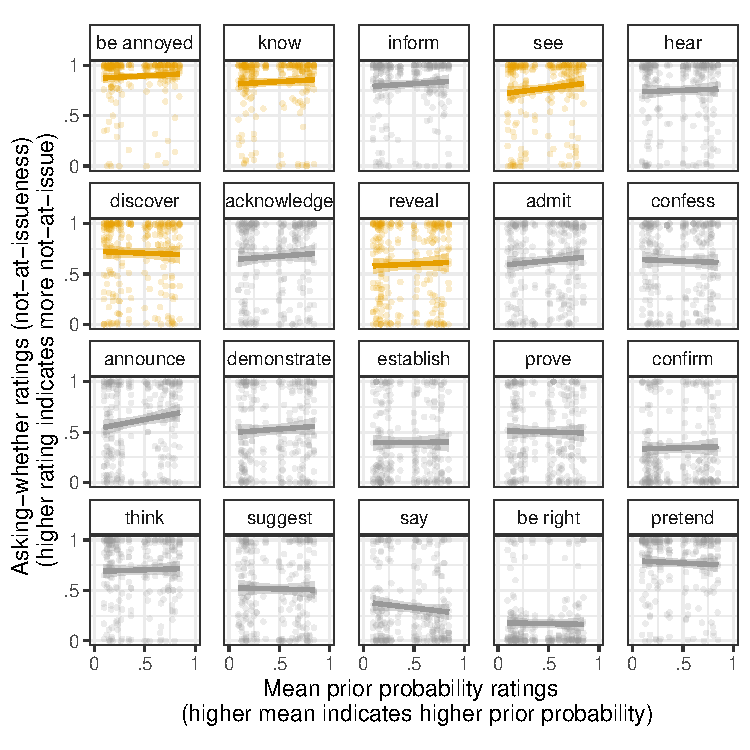
\includegraphics[width=.9\textwidth]{../../results/main/exp1/graphs/SUP-aiproj-ai-by-prior}
\caption{Ai/proj dataset.}
 \end{subfigure}
 
  
\caption{Participants' asking-whether ratings (measuring at-issueness) against prior probability ratings in Exp.~1: (a) Proj/ai dataset, (b) Ai/proj dataset. Linear smoothers with 95\% confidence intervals overlaid. Predicates are ordered by projection mean, with purportedly factive predicates in orange.}
\end{figure}

\subsection{Certainty ratings against asking-whether ratings by prior probability}

\begin{figure}[h!]
\centering
\begin{subfigure}[t]{0.49\textwidth}
\centering
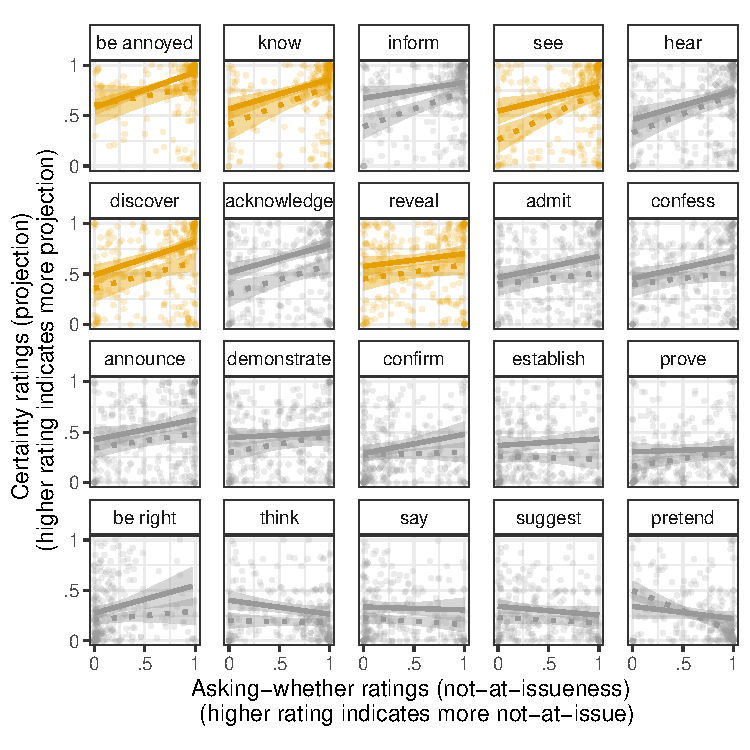
\includegraphics[width=.9\textwidth]{../../results/main/exp1/graphs/SUP-projai-projection-by-ai-and-prior}
\caption{Proj/ai dataset.}
\end{subfigure} \hfill \begin{subfigure}[t]{0.49\textwidth}
\centering
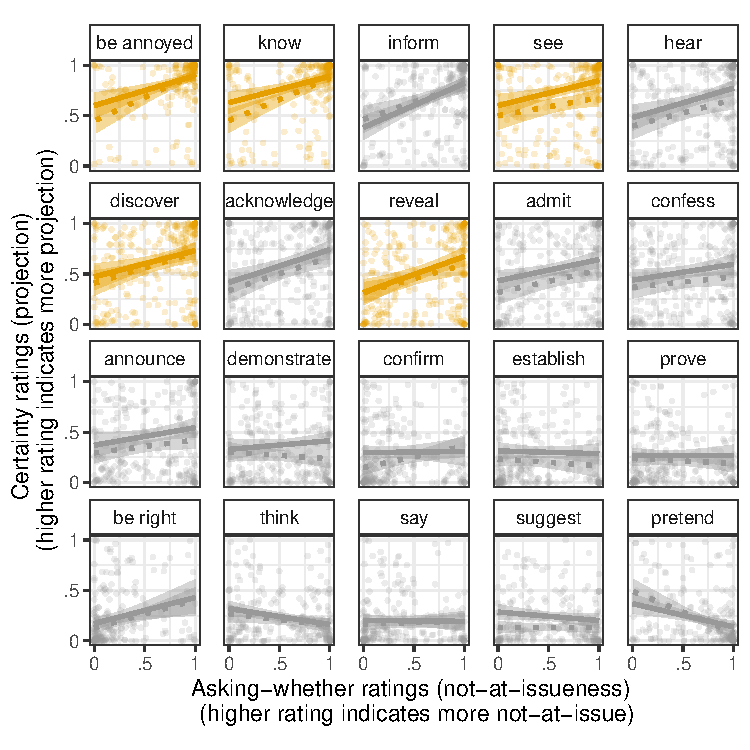
\includegraphics[width=.9\textwidth]{../../results/main/exp1/graphs/SUP-aiproj-projection-by-ai-and-prior}
\caption{Ai/proj dataset.}
 \end{subfigure}
 
  
\caption{Participants' certainty ratings (measuring projection) against asking-whether ratings (measuring at-issueness) by high (solid line: ---) and low prior probability fact (dotted line: \raisebox{1mm}{\ldots}) in Exp.~1: (a) Proj/ai dataset, (b) Ai/proj dataset. Linear smoothers with 95\% confidence intervals overlaid Predicates are ordered by projection mean, with purportedly factive predicates in orange.}
\end{figure}

\newpage

\section{Comparison of ratings across experiments}

\subsection{Comparisons of by-predicate projection variation}\label{a-replication}

The mean certainty ratings of the predicates in the experiment reported  in this paper are compared in Fig.~\ref{fig:comparison-language} to those of Exp.~1 of \citealt{degen-tonhauser-language} (abbreviated `Exp 1 DT in print') and, in Fig.~\ref{fig:comparison-openmind}, to those of  Exp.~1 of \citealt{degen-tonhauser-openmind} (abbreviated `Exp 1 DT 2021'). 

\begin{figure}[h!]
\centering
\begin{subfigure}[t]{0.5\textwidth}
        \centering
%\includegraphics[width=.3\paperwidth]{../../results/main/exp1/graphs/projection-comparison-with-DT-Language}
\caption{}\label{fig:comparison-language}
 \end{subfigure}%
\begin{subfigure}[t]{0.5\textwidth}
\centering
%\includegraphics[width=.3\paperwidth]{../../results/main/exp1/graphs/projection-comparison-with-DT-OpenMind}
\caption{}\label{fig:comparison-openmind}
\end{subfigure}
\caption{Comparisons of mean by-predicate certainty ratings from the experiment reported on in this paper and Exp.~1 from \citealt{degen-tonhauser-openmind} (abbreviated `Exp 1 DT 2021'). Error bars indicate 95\% bootstrapped confidence intervals.} 
\label{f-comparison}
\end{figure}

\subsection{Comparisons of prior belief ratings in Exps.~1, DT1, and DT2a}\label{a-beliefs-corr-prior}

\begin{figure}[h!]
\centering
\begin{subfigure}[t]{.3\textwidth}
\centering
\includegraphics[width=\textwidth]{../../results/expsDT12/graphs/prior-exp1-expDT1}
\caption{Exp.~1 against Exp.~DT1}\label{fig:prior-exp1-expDT1}
\end{subfigure} \hfill \begin{subfigure}[t]{.3\textwidth}
\centering
\includegraphics[width=\textwidth]{../../results/expsDT12/graphs/prior-exp1-expDT2a}
\caption{Exp.~1 against Exp.~DT2.}\label{fig:prior-exp1-expDT2a}
 \end{subfigure} \hfill \begin{subfigure}[t]{.3\textwidth}
\centering
\includegraphics[width=\textwidth]{../../results/expsDT12/graphs/prior-expDT1-expDT2a}
\caption{Exp.~DT1 against Exp.~DT2}\label{fig:prior-expDT1-expDT2a}
 \end{subfigure}
\caption{Comparisons of the 40 by-content/fact mean prior probability ratings in Exps.~1, DT1, and DT2a.}
\end{figure}

\newpage

\subsection{Comparisons of at-issueness ratings in Exps.~1 and 2}\label{a-beliefs-corr-ai}

\begin{figure}[h!]
\centering
\begin{subfigure}[t]{.45\textwidth}
\centering
\includegraphics[width=\textwidth]{../../results/expsDT12/graphs/ai-by-PCF-exp1-exp2}
\caption{By content/fact/predicate (judgments: 4-27, mean: 12)}
\end{subfigure} \hfill \begin{subfigure}[t]{.45\textwidth}
\centering
\includegraphics[width=\textwidth]{../../results/expsDT12/graphs/ai-by-PC-exp1-exp2}
\caption{By content/predicate (judgments: 14-43, mean: 25)}

\begin{subfigure}[t]{.4\textwidth}
\centering
\includegraphics[width=\textwidth]{../../results/expsDT12/graphs/ai-by-CF-exp1-exp2}
\caption{By content/fact)}
 \end{subfigure} \hfill \begin{subfigure}[t]{.4\textwidth}
\centering
\includegraphics[width=\textwidth]{../../results/expsDT12/graphs/ai-by-P-exp1-exp2}
\caption{By predicate (500-505 judgments)}
 \end{subfigure}
 \end{subfigure}
 
\caption{Comparisons of the mean asking-whether ratings in Exps.~1 and 2.}\label{fig:ai-comparisons}
\end{figure}

\section{Bayesian model outputs}\label{a-models}

\subsection{Experiment 1}\label{a-models-exp1}

\input{../../results/main/exp1/models/latex-tables/exp1.model}

\subsection{Experiment 2}\label{a-models-exp2}

\input{../../results/main/exp2/models/latex-tables/exp2.model}

\subsection{Experiment DT1 and DT2}\label{a-models-OM}

\input{../../results/expsDT12/models/latex-tables/OMExp-Bayesian}



\end{document}

